
\documentclass[11pt]{beamer}
% \usepackage[round]{natbib}
\usetheme{TUD}
\usepackage{svg}
\usepackage[utf8]{inputenc}
\usepackage{booktabs}
\usepackage{multicol}
\usepackage{multirow}
\usepackage{graphicx}
\usepackage[T1]{fontenc}
\usepackage{color}
\usepackage{caption}
\usepackage{amsmath}
\usepackage{bm}
\usepackage{listings}
\captionsetup[table]{position=bottom}

% Dark Colors
\definecolor{deepblue}{rgb}{0.2980392156862745, 0.4470588235294118, 0.6901960784313725}
\definecolor{deepgreen}{rgb}{0.3333333333333333, 0.6588235294117647, 0.40784313725490196}
\definecolor{deepred}{rgb}{0.7686274509803922, 0.3058823529411765, 0.3215686274509804}
\definecolor{deeplightblue}{rgb}{0.39215686274509803, 0.7098039215686275, 0.803921568627451}

% Light colors
\definecolor{lightblue}{rgb}{0.6509803921568628, 0.807843137254902, 0.8901960784313725}
\definecolor{lightgreen}{rgb}{0.6980392156862745, 0.8745098039215686, 0.5411764705882353}
\definecolor{lightred}{rgb}{0.984313725490196, 0.6039215686274509, 0.6}
\definecolor{lightgrey}{rgb}{0.8019607843137254, 0.8019607843137254, 0.8019607843137254}


\newenvironment{wideitemize}{\itemize\addtolength{\itemsep}{.75em}}{\enditemize}
\newenvironment{wideenumerate}{\enumerate\addtolength{\itemsep}{.75em}}{\endenumerate}

\newcommand{\addsubitemspace}{\vspace{0.5em}}

% Default fixed font does not support bold face
\DeclareFixedFont{\ttb}{T1}{txtt}{bx}{n}{12} % for bold
\DeclareFixedFont{\ttm}{T1}{txtt}{m}{n}{12} % for normal


\begin{document}
\author{Fabian Kessler, Dominik Straub, Steven Lang}
\title{Monocular Depth Estimation Using Atrous Convolutions}
\subtitle{Supervisor: Faraz Saeedan\\Group 5} %TODO where to put Faraz?
% \logo{"tud\_logo".png} \institute{Technische Universit\"at Darmstadt}
\date{February 18, 2019}
% \subject{} \setbeamercovered{transparent} \setbeamertemplate{navigation % symbols}{}
\maketitle

% Lstset colors
\definecolor{mygreen}{rgb}{0,0.6,0} \definecolor{mygray}{rgb}{0.5,0.5,0.5}
\definecolor{mymauve}{rgb}{0.58,0,0.82}

\lstset{ %
  backgroundcolor=\color{white}, % choose the background color; you must add \usepackage{color} or \usepackage{xcolor}
  basicstyle=\ttfamily\footnotesize, % the size of the fonts that are used for the code
  breakatwhitespace=false, % sets if automatic breaks should only happen at whitespace
  breaklines=true, % sets automatic line breaking
  captionpos=b, % sets the caption-position to bottom
  commentstyle=\color{mygreen}, % comment style
  deletekeywords={...}, % if you want to delete keywords from the given language
  escapeinside={(*@}{@*)}, % if you want to add LaTeX within your code
  extendedchars=true, % lets you use non-ASCII characters; for 8-bits encodings only, does not work with UTF-8
  % frame=single, % adds a frame around the code
  keepspaces=true, % keeps spaces in text, useful for keeping indentation of code (possibly needs columns=flexible)
  % keywordstyle=\color{blue}, % keyword style
  language=Python, % the language of the code
  % otherkeywords={*,...}, % if you want to add more keywords to the set
  numbers=none, % where to put the line-numbers; possible values are (none, left, right)
  numbersep=-3pt, % how far the line-numbers are from the code
  numberstyle=\tiny\color{mygray}, % the style that is used for the line-numbers
  % rulecolor=\color{black}, % if not set, the frame-color may be changed on line-breaks within not-black text (e.g. comments (green here))
  showspaces=false, % show spaces everywhere adding particular underscores; it overrides 'showstringspaces'
  showstringspaces=false, % underline spaces within strings only
  showtabs=false, % show tabs within strings adding particular underscores
  stepnumber=1, % the step between two line-numbers. If it's 1, each line will be numbered
  % stringstyle=\color{mymauve}, % string literal style
  tabsize=2, % sets default tabsize to 2 spaces
  % title=\lstname % show the filename of files included with \lstinputlisting; also try caption instead of title
  escapeinside=||, } \newcommand{\argmax}{\operatornamewithlimits{argmax}}
\newcommand{\amax}{\operatornamewithlimits{max}}

\setbeamerfont{footnote}{size=\tiny} \newcommand{\specialcell}[2][c]{%
  \begin{tabular}[#1]{@{}l@{}}#2\end{tabular}}

\newcommand\Wider[2][3em]{%
  \makebox[\linewidth][c]{%
    \begin{minipage}{\dimexpr\textwidth+#1\relax}
      \raggedright#2
    \end{minipage}%
  }%
}

\addtocounter{framenumber}{-1}

\setcounter{tocdepth}{1} % define depth of toc

% TOC FRAME
\begin{frame}[allowframebreaks]
  \tableofcontents
\end{frame}%[pausesections]}

% Start content
\section{Introduction}
\label{sec:orgd88665b}

\subsection{Monocular Depth Estimation}
\label{sec:org3a87c71}
\begin{frame}[c]{Monocular Depth Estimation}

    \begin{columns}
        \begin{column}{0.6\textwidth}
        \begin{wideitemize}
        \item Monodepth: Estimate depth from a single image at test-time (instead of stereo pair)
        \item Existing approaches treat this as a supervised regression problem
        \item Godard et al., CVPR 2017: Depth estimation as a stereo reconstruction problem
        \end{wideitemize}
        \end{column}
        \begin{column}{0.4\textwidth}
        \centering
          \begin{figure}
          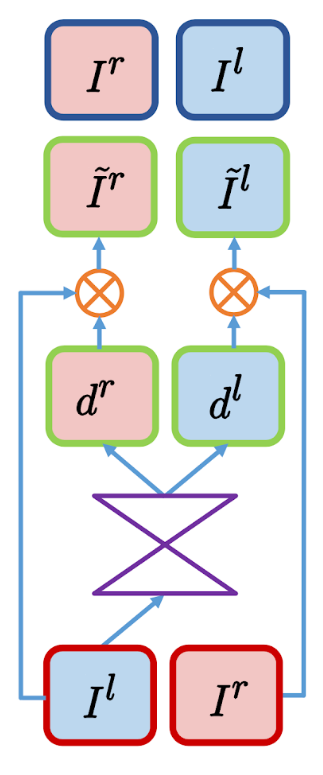
\includegraphics[height=.75\textheight]{figures/monodepth.png}
          \caption{Godard et al. 2017}
          \end{figure}
        \end{column}
        
    \end{columns}

\end{frame}

\subsection{Atrous Convolutions}
\begin{frame}[c]{Atrous Convolutions}
\begin{figure}
    \centering
    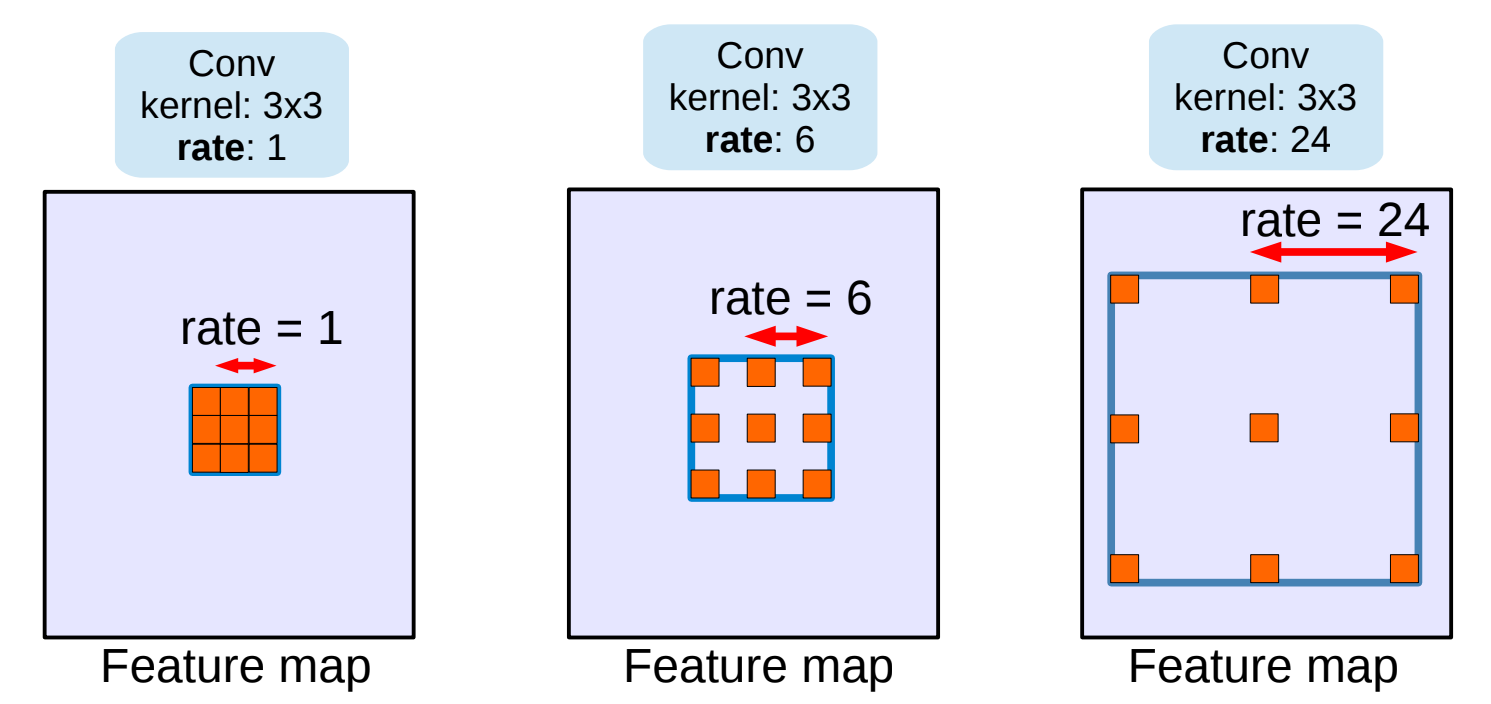
\includegraphics[width=1.0\textwidth]{figures/atrous_conv.png}
    \caption{Chen et al., 2017}
\end{figure}

\end{frame}



\section{Experiments \& Results}

\begin{frame}[c]{Project Objective}
  \begin{wideitemize}
  \item Get Monodepth baseline to run
  \item Design and implement encoder-decoder network using atrous convolutions
  \item Consider memory and runtime in architectural decisions
  \item Quantitative comparison of proposed architectures to baseline
  \end{wideitemize}
\end{frame}

\subsection{Our Project}
\begin{frame}[c]{Our Architecture with ASPP}
  \centering
  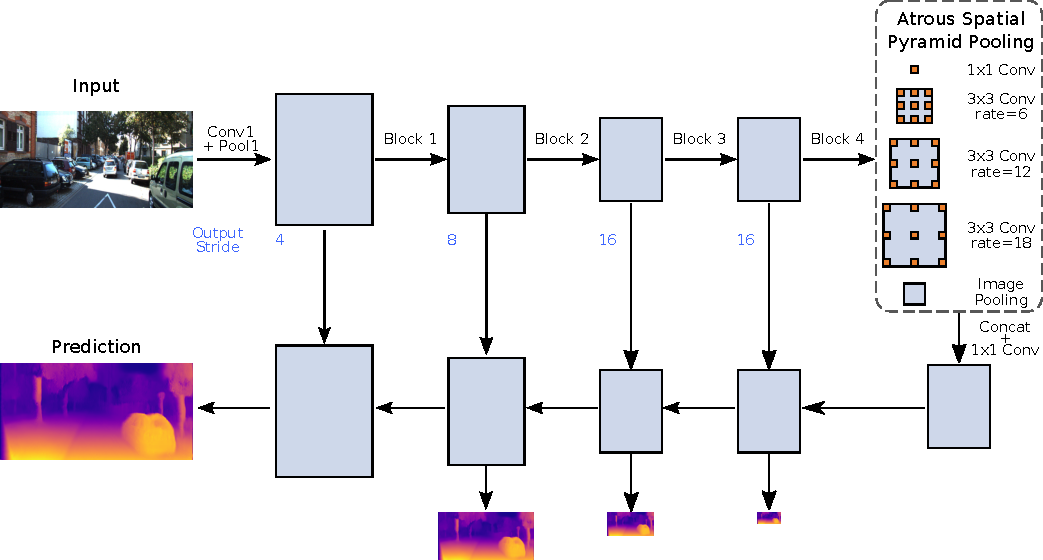
\includegraphics[width=1.0\textwidth]{figures/architecture/architecture.pdf}
\end{frame}


\subsection{Remember last time? Sky Artifacts}
\label{sec:orgcd1d83a}
\begin{frame}[c]{\subsecname}
  \centering
  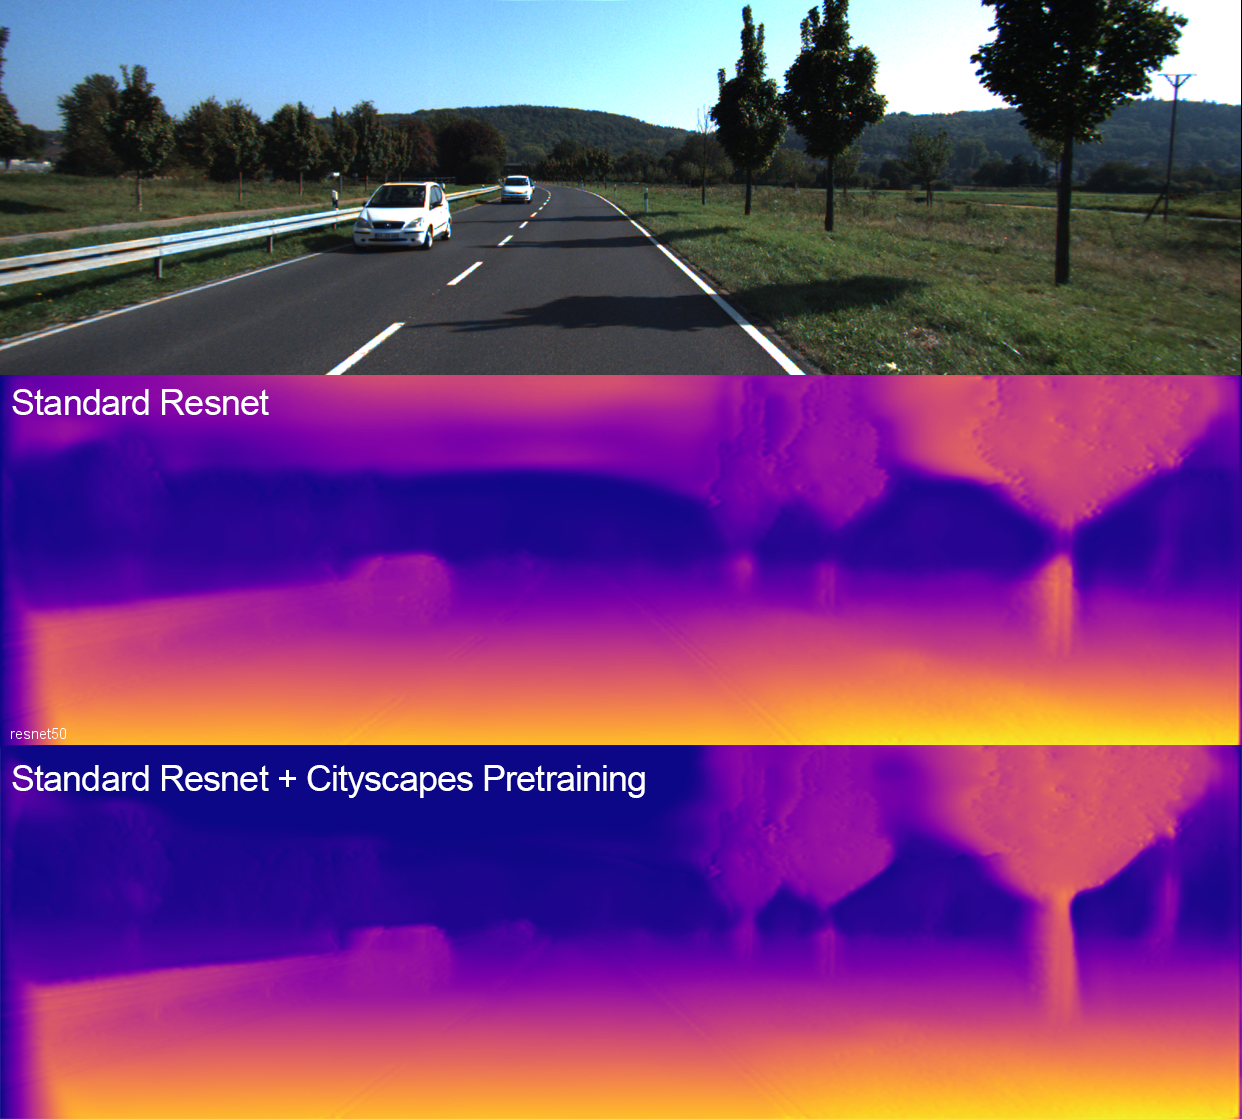
\includegraphics[width=0.7\textwidth]{figures/images/implementationcomparison_004.png}
\end{frame}


\begin{frame}[c]{How we solved it: Reimplementation}
\begin{center}
  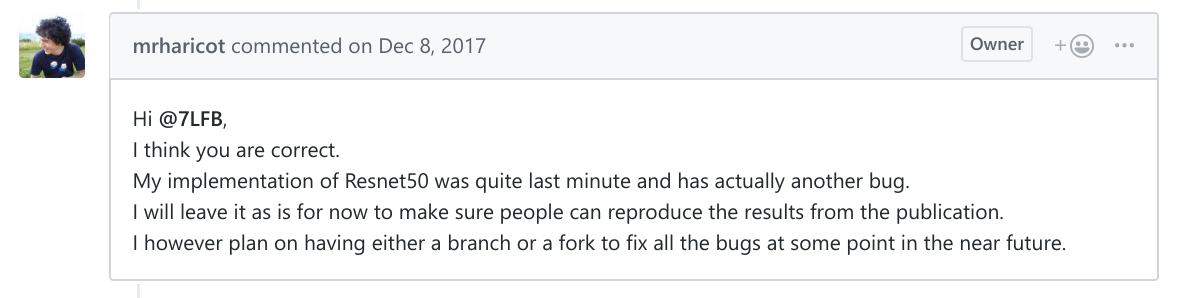
\includegraphics[width=0.9\textwidth]{figures/godard-github.png}
\end{center}

% TODO-START: Skip this sentence (too much on the slide) ? %
%Surprisingly, a standard (\texttt{torchvision}) implementation of ResNet-50 also produced the sky-artifacts..
% TODO-END %
\pause
\vfill

Differences of their implementation compared to standard ResNet:
\addsubitemspace
  \begin{wideitemize}
  \item No batch-normalization
  \item Nearest-neighbor instead of bilinear interpolation
  \item Order of convolution strides in ResNet switched
  \end{wideitemize}
\vfill
  {\color{tudred}+} Fixed bug in author's implementation of loss function
\end{frame}

\begin{frame}[c]{New Disparity Maps}
\centering
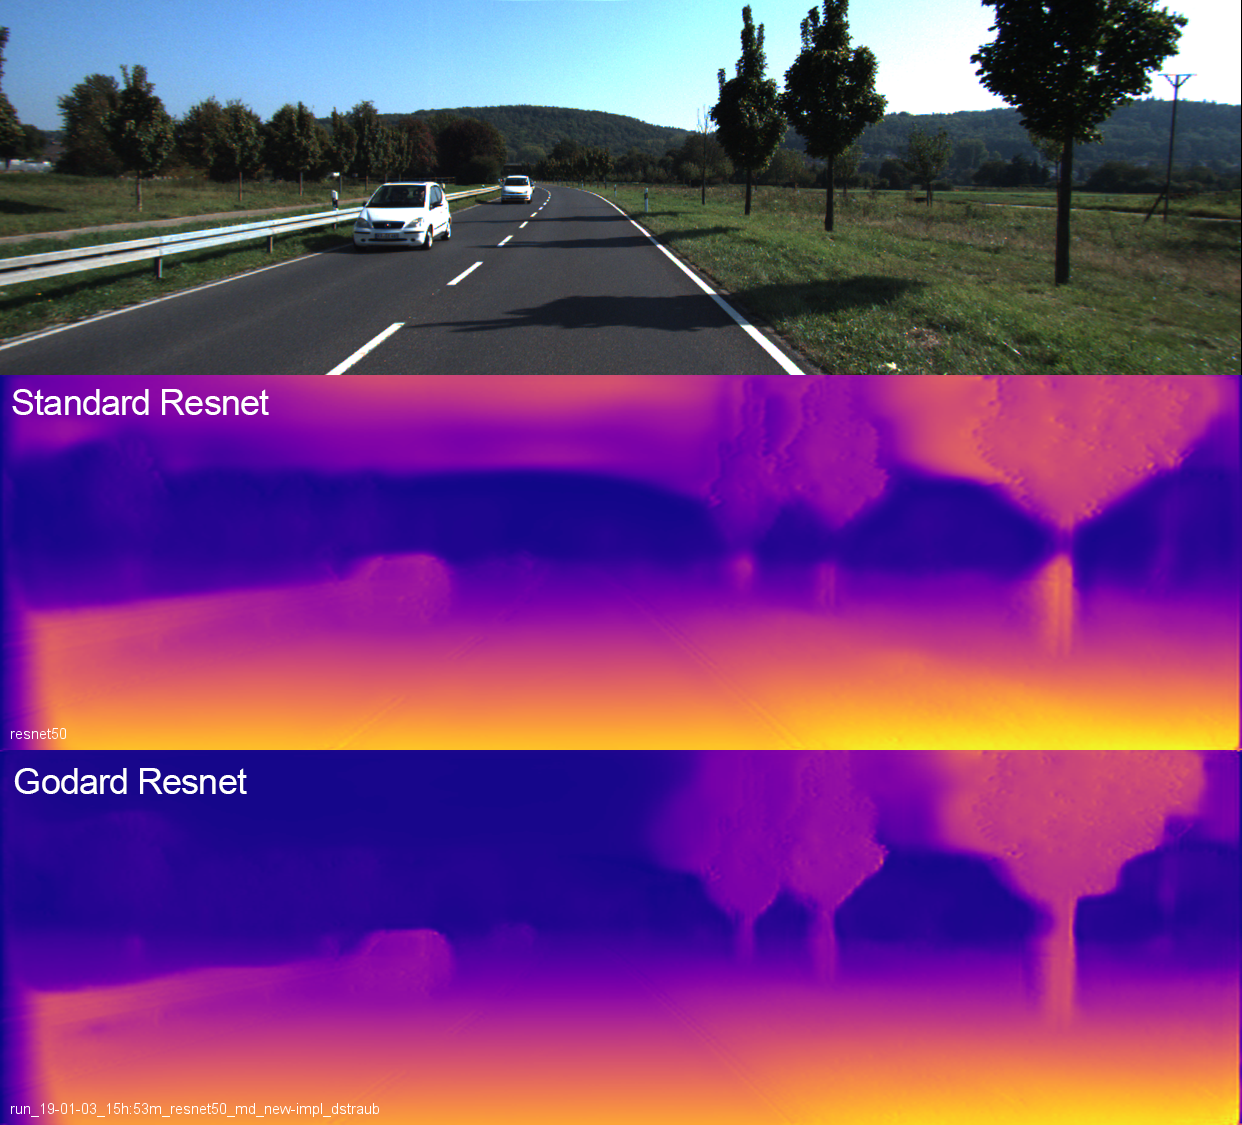
\includegraphics[width=0.7\textwidth]{figures/images/implementationcomparison_001.png}
\end{frame}


\subsection{Experiments}
\begin{frame}[c]{General Experimental Setup}
  
    \begin{columns}
        \begin{column}{0.5\textwidth}
           \begin{wideitemize}
            \item General setup
            \addsubitemspace
            \begin{wideitemize}
                \item Batch Size 16
                \item Learning Rate 2e-4
                \item 50 epochs
            \end{wideitemize}
            
            \item KITTI for training        
            \addsubitemspace
                \begin{wideitemize}
                    \item Rescaled to 256 x 512 px
                \end{wideitemize}
            \item KITTI Stereo 2015 for testing
            \addsubitemspace
                \begin{wideitemize}
                    \item Sparse ground truth
                \end{wideitemize}
            \end{wideitemize}
        \end{column}
        
        % TODO: Shouldn't we show an example and its ground truth instead of two unrelated images?
        \begin{column}{0.5\textwidth}
            \centering
            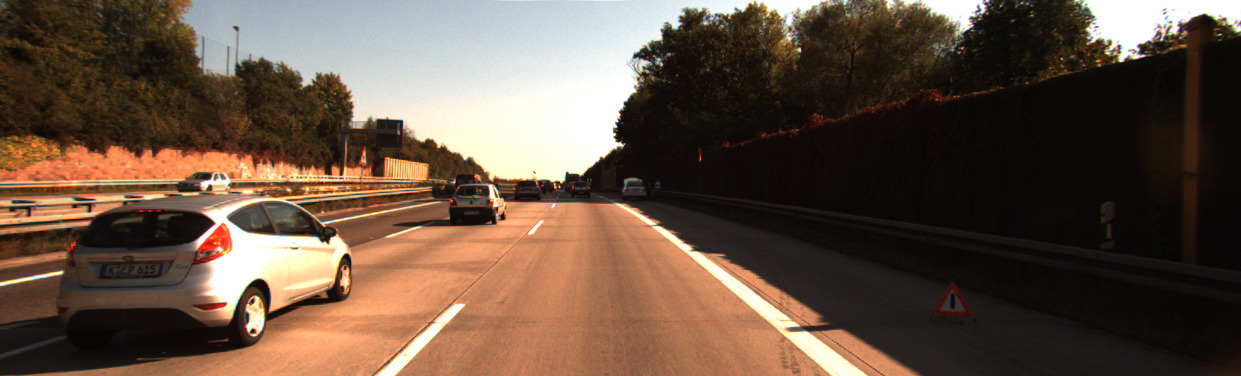
\includegraphics[width=1.0\textwidth]{figures/kitti_example.jpg}
            
            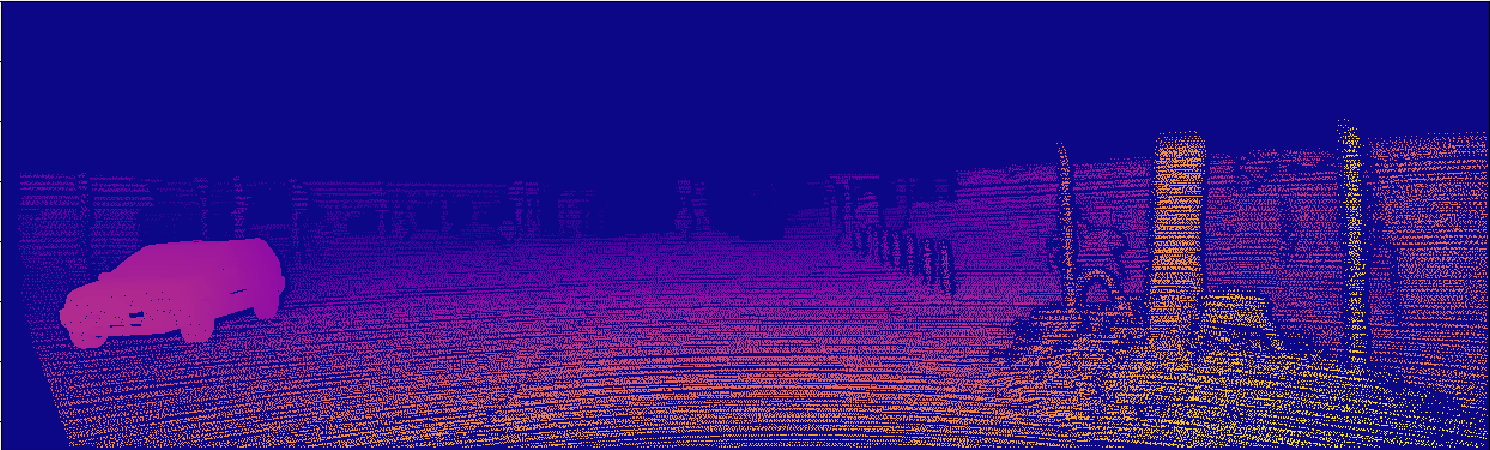
\includegraphics[width=1.0\textwidth]{figures/kitti_gt.png}

        \end{column}
   \end{columns}
\end{frame}

\begin{frame}[c]{\subsecname: Output Strides}{Issues}
  Output stride 64 with Atrous rate > 1
  \begin{center}
    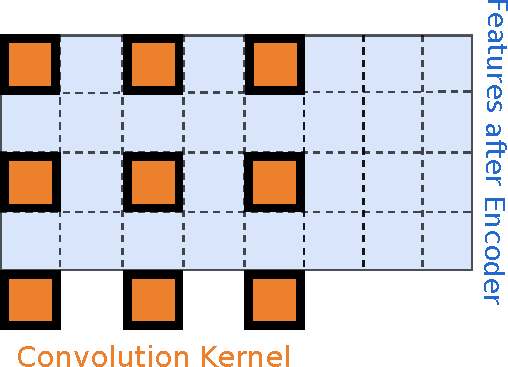
\includegraphics[width=0.7\textwidth]{figures/architecture/os64-atrous-conv-with-text.pdf}
  \end{center}
\end{frame}

\begin{frame}[c]{Experiments: Output Strides}
\centering
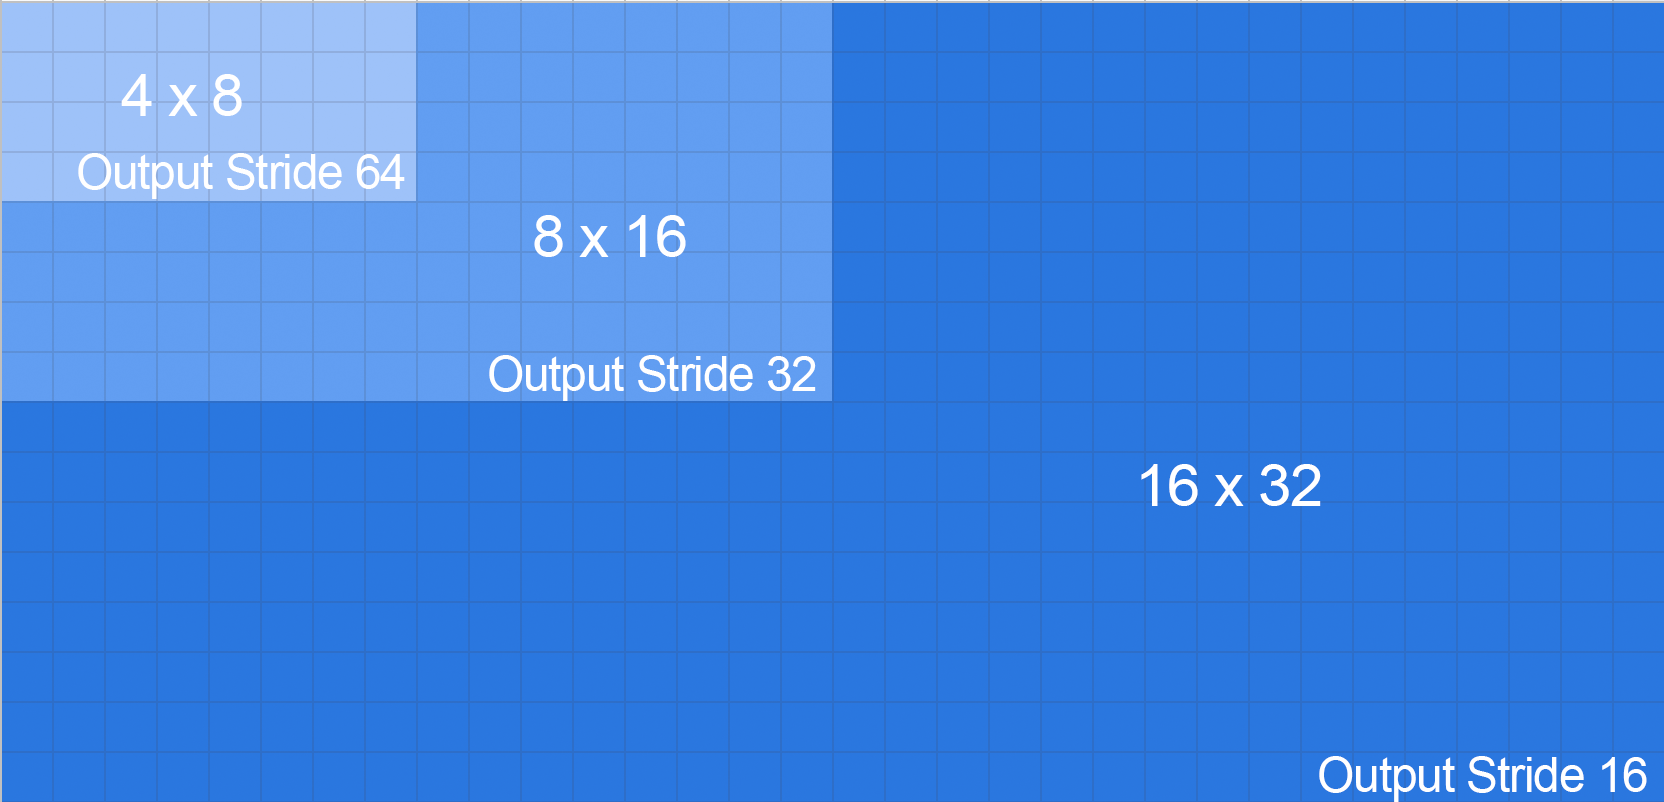
\includegraphics[width=0.7\textwidth]{figures/images/output_stride_text.png}
\vfill
\pause
\begin{tabular}{rrrrr}
\toprule
Stride &  Abs. Rel. & Runtime {\tiny $\left(\frac{Min.}{Epoch}\right)$} & Memory (GB) & Param. (M) \\
\midrule
64 &    0.1120 & \textbf{15}  &     \textbf{6.12} &  58.4 \\
32 &    0.1048 &  29  &     8.87 &  58.4 \\
16 &    \textbf{0.1041} &  29  &     8.88 &  58.4 \\
8 &     0.1068 &  43  &    10.61 &  58.4 \\
\bottomrule
\end{tabular}

\end{frame}

\begin{frame}[c]{\subsecname: ASPP vs. no ASPP}
\centering
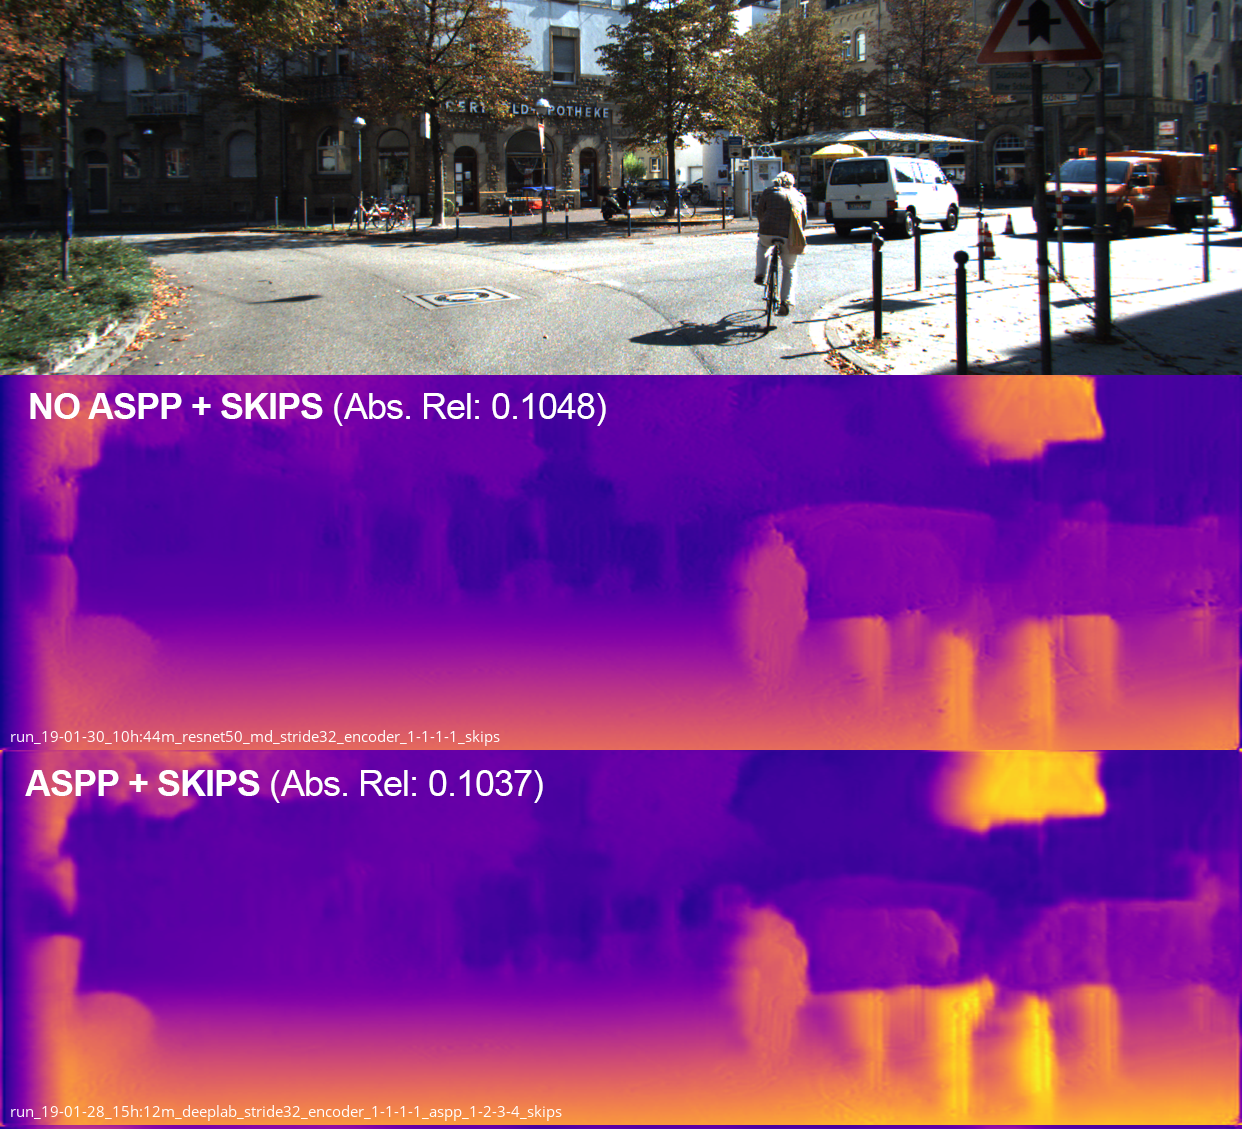
\includegraphics[width=0.7\textwidth]{figures/images/skipsvsnoskips1_error.png}
\end{frame}



\begin{frame}[c]{\subsecname: Atrous Rates}
    \begin{columns}
            \begin{column}{0.3\textwidth}
            \centering
            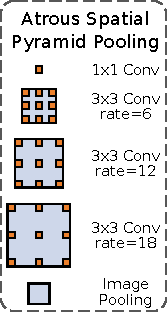
\includegraphics[width=0.7\textwidth]{figures/architecture/aspp-module.pdf}
            \end{column}%
            \pause
            \begin{column}{0.8\textwidth}
            \centering
  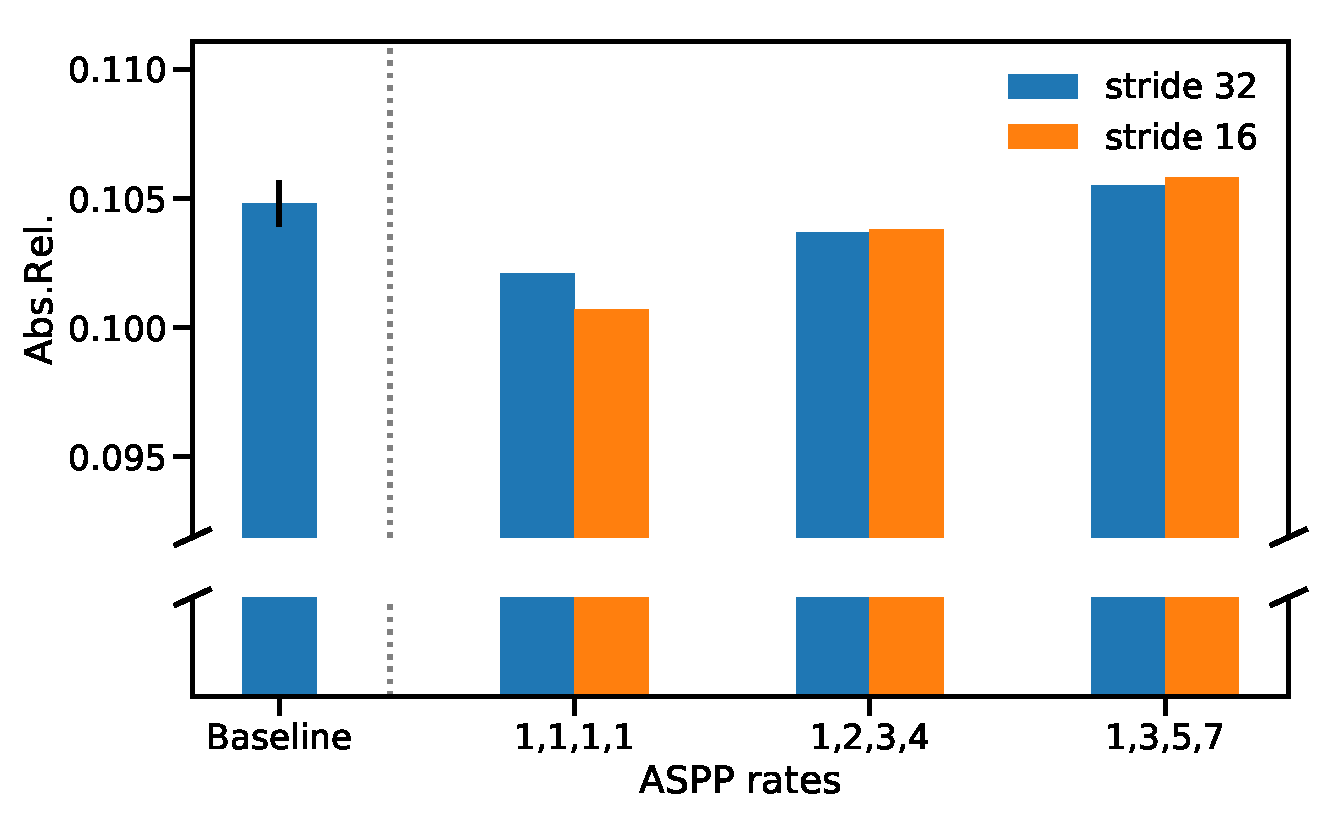
\includegraphics[width=1.0\textwidth]{figures/results/experiment1_AbsRel.pdf}
            \end{column}
    \end{columns}
  
\end{frame}

\begin{frame}[c]{\subsecname: Different Number of Modules}
    \begin{columns}
            \begin{column}{0.3\textwidth}
            \centering
            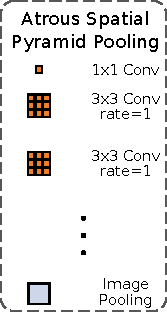
\includegraphics[width=0.7\textwidth]{figures/architecture/aspp-module-dynamic.pdf}
            \end{column}%
            \pause
            \begin{column}{0.8\textwidth}
              \centering
              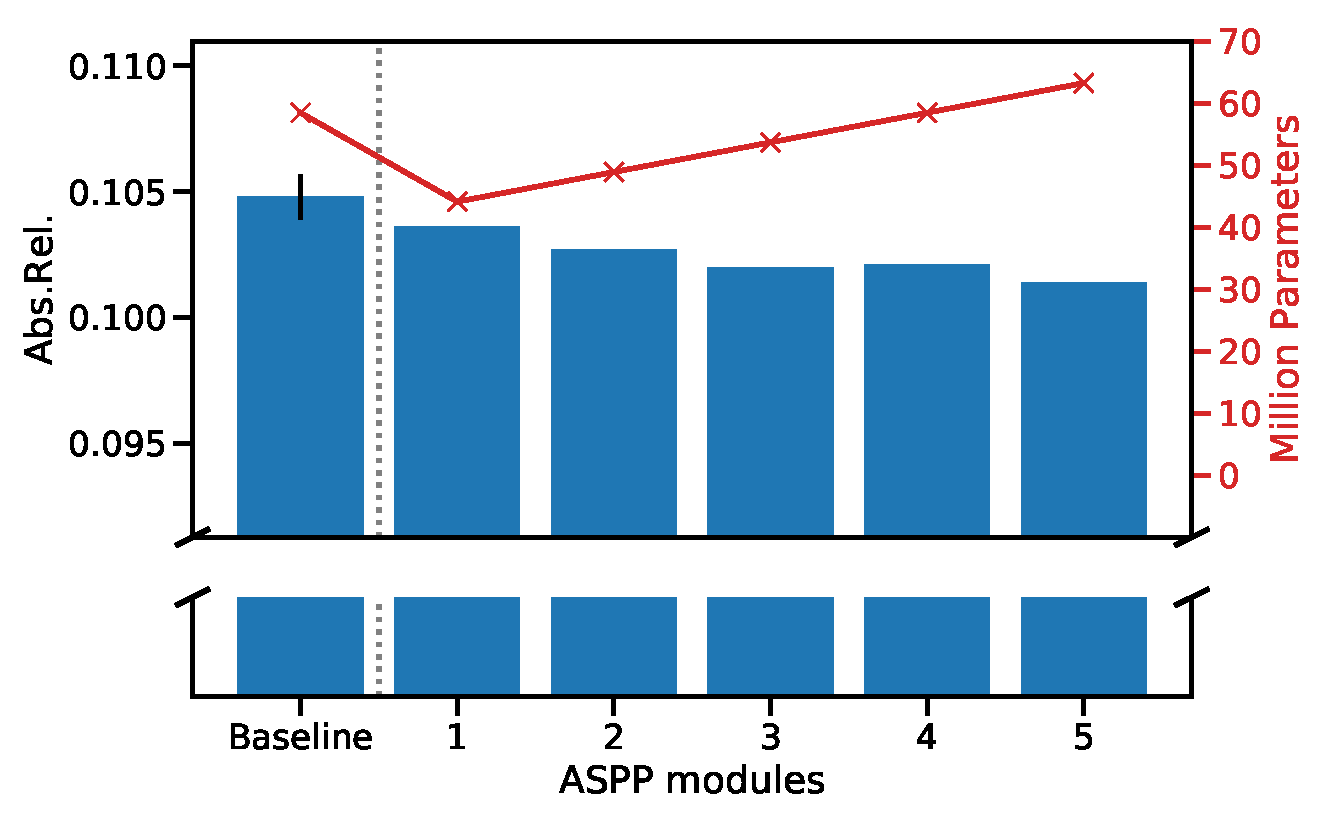
\includegraphics[width=1.0\textwidth]{figures/results/experiment2_AbsRel.pdf}
            \end{column}
    \end{columns}
\end{frame}

\begin{frame}[c]{\subsecname: Atrous Convolutions in Encoder}
  \centering
   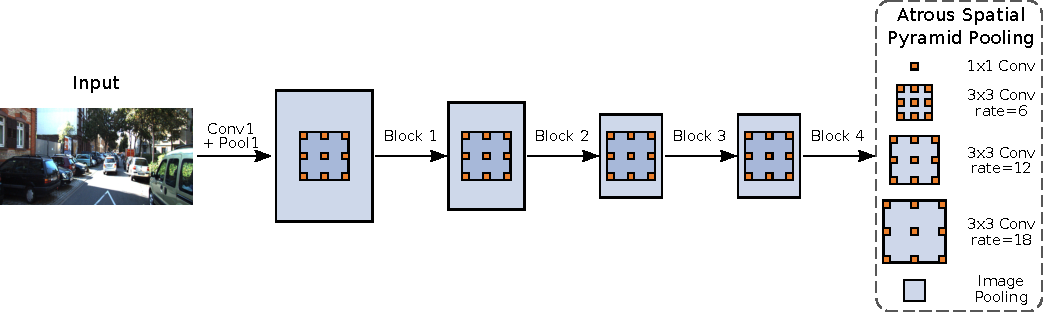
\includegraphics[width=1.0\textwidth]{figures/architecture/encoder-with-atrous-rates.pdf}
   \vfill
   No improvement with atrous convolutions in ResNet blocks
\end{frame}

\begin{frame}[c]{\subsecname: ASPP in ResNet}
  \centering
  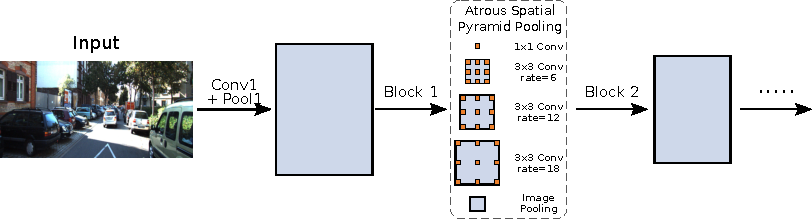
\includegraphics[width=1.0\textwidth]{figures/architecture/aspp-in-encoder.pdf}
  \vfill
  No improvement with ASPP module between ResNet blocks
\end{frame}

\begin{frame}[c]{Final Results}{Pretrained on CityScapes \& finetuned on KITTI}
 \centering
 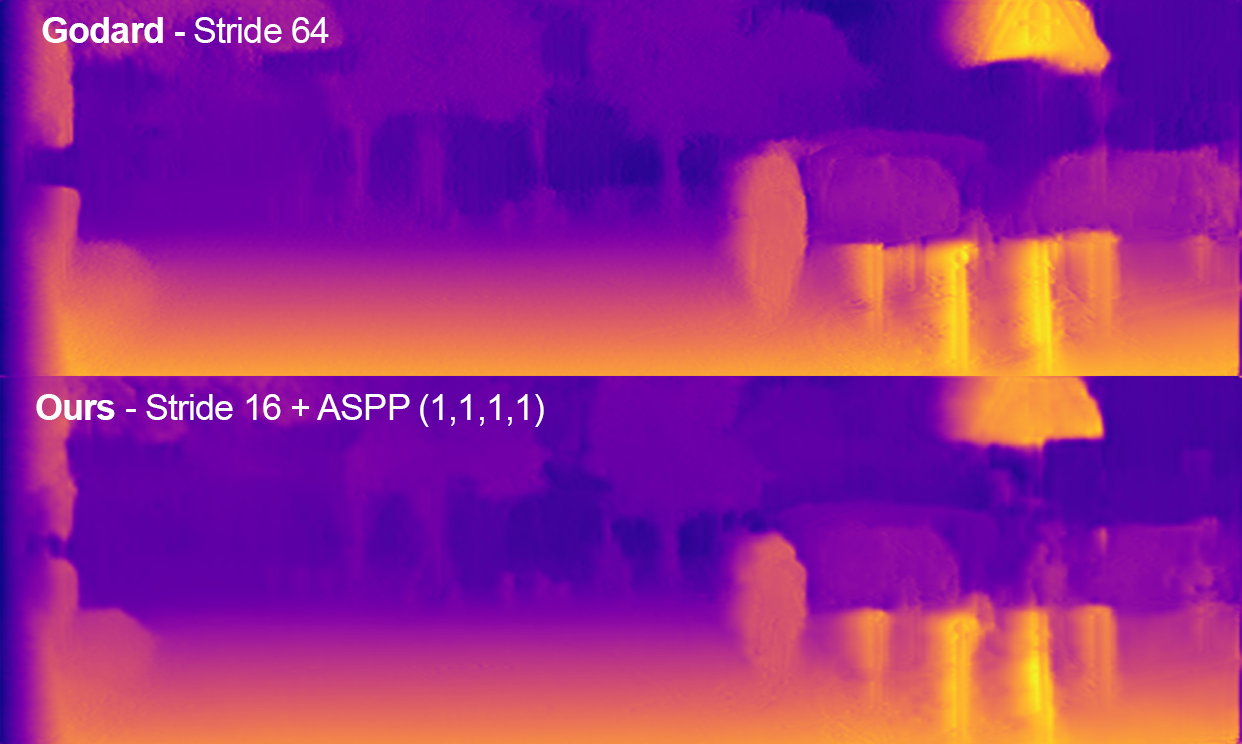
\includegraphics[width=0.7\textwidth]{figures/images/final_godard_comparison.png}
 \vfill
 \scalebox{.5} {
 \begin{tabular}{lllrrrrrrrrr}
\toprule
 Output-stride &     ASPP &  Abs.Rel. &  Sq.Rel. &   RMSE &  Log RMSE &     a1 &     a2 &     a3 &      Params (M) & $\Delta$ Abs. Rel. (\%)\\
\midrule
       64 - Godard &      - &    0.0970 &   0.8960 &  5.093 &     0.176 &  0.962 &  0.962 &  0.986 &         58.4 & -- \\
       16 - Godard & - & 0.0955 & 0.8752 &      4.937 &      0.174 &     0.881 &      0.961 &    0.984 & 58.4 & 2.57 \\
            16 - Ours &  1-1-1-1 &    \textbf{0.0927} &   \textbf{0.8132} &  \textbf{4.865} &     \textbf{0.168} &  \textbf{0.888} &  \textbf{0.967} &  \textbf{0.987} &         58.4 & \textbf{4.43} \\
            32 - Ours &   1 &    0.0941 &   0.8196 &  4.910 &     0.173 &  0.882 &  0.963 &  0.986 &         \textbf{44.1} & 2.99 \\
            32 - Ours &  1-2-3-4 &    0.0936 &   0.8281 &  4.941 &     0.172 &  0.884 &  0.963 &  \textbf{0.987} &         58.4 & 3.50\\
\bottomrule
\end{tabular}

 }
\end{frame}

\section{Discussion}
\begin{frame}[c]{\secname}
    \begin{wideitemize}
        \item Hyperparameter tuning
        \addsubitemspace
        \begin{wideitemize}
        \item Learning rate
        \item Loss hyperparameters
        \begin{align*}
            C_s = \boldsymbol{\alpha_{ap}}\left(C^l_{ap} + C^r_{ap}\right) + \boldsymbol{\alpha_{ds}}\left(C^l_{ds} + C^r_{ds}\right) + \boldsymbol{\alpha_{lr}}\left(C^l_{lr} + C^r_{lr}\right)
        \end{align*}
        
        \item Focus on architectural design instead
        \end{wideitemize}
    \end{wideitemize}
\end{frame}
\begin{frame}[c]{\secname}
\begin{wideitemize}
        \item Output stride 8
        \item Decoder architecture
        \item Robustness of training \& predictions
\end{wideitemize}

\end{frame}

\section{Conclusion}
\begin{frame}[c]{Recap}
  \begin{wideitemize}
  \item Reproduced baseline
  \item Experiments
  \vspace{0.75em}
  \begin{wideitemize}
  \item Output stride
  \item ASPP rates
  \item Number of ASPP modules
  \item Atrous convolutions in encoder
  \end{wideitemize}
  \end{wideitemize}
\end{frame}
\begin{frame}[c]{\secname}
    \begin{wideitemize}
      \item Atrous convolutions \dots
      \addsubitemspace
      \begin{wideitemize}
      \item do not improve monocular depth estimation
      \item need a decreased output stride, which harms runtime and memory
      \end{wideitemize}
  \item Channel reduction after encoder \dots
  \addsubitemspace
  \begin{wideitemize}
  %\item improves prediction performance
  \item decreases parameter count and improves runtime
  \item without losing predictive power
  \end{wideitemize}
  \end{wideitemize}
\end{frame}

\begin{frame}[c]{References}
    \begin{wideitemize}
    \item C. Godard, O. Aodha and G. Brostow: Unsupervised Monocular Depth Estimation with Left- Right Consistency, CVPR 2017.
    \item L. Chen, Y. Zhu, G. Papandreou, F. Schroff, H. Adam: Encoder-Decoder with Atrous Separable Convolution for Semantic Image Segmentation. arXiv 2018.
    \item M. Cordts, M. Omran, S. Ramos, T. Rehfeld, M. Enzweiler, R. Benenson, U. Franke, S. Roth, B. Schiele: The cityscapes dataset for semantic urban scene understanding. CVPR. 2016.
    \item M. Menze and A. Geiger: Object Scene Flow for Autonomous Vehicles. CVPR. 2015. 
    \end{wideitemize}
\end{frame}

\section*{Backup slides}
% Experiment 1 result metric
\begin{frame}[c]{\subsecname: Atrous Rates (Visual Comparison)}
  \centering
  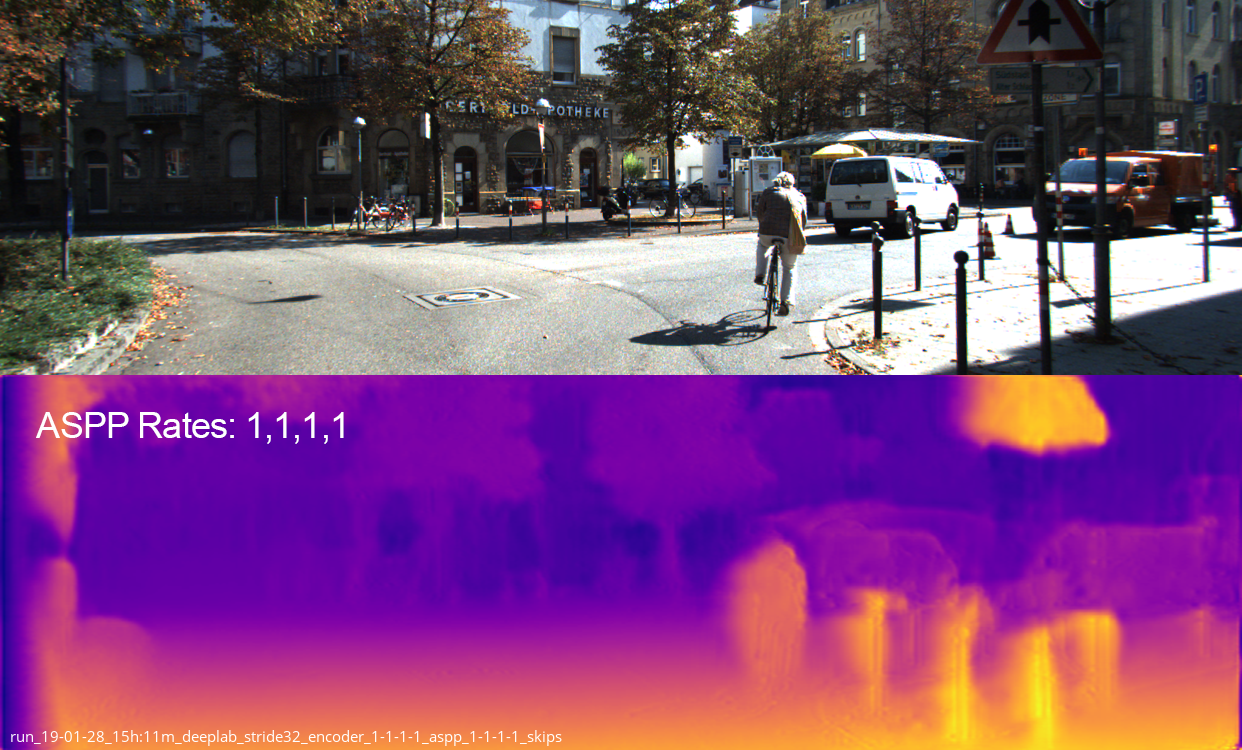
\includegraphics[width=1.0\textwidth]{figures/images/asppcomparison_001.png}
\end{frame}

\begin{frame}[c]{\subsecname: Atrous Rates (Visual Comparison)}
  \centering
  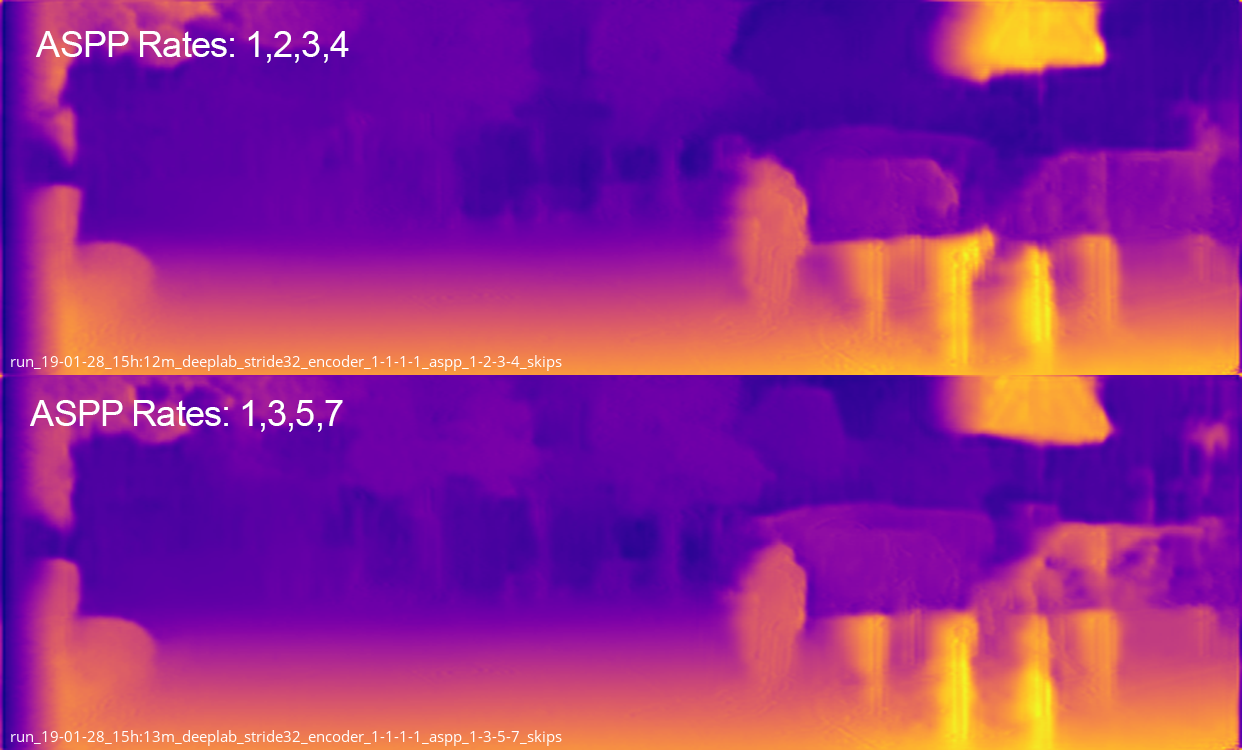
\includegraphics[width=1.0\textwidth]{figures/images/asppcomparison_002.png}
\end{frame}

\begin{frame}[c]{\subsecname: Atrous Rates (Visual Comparison)}
  \centering
  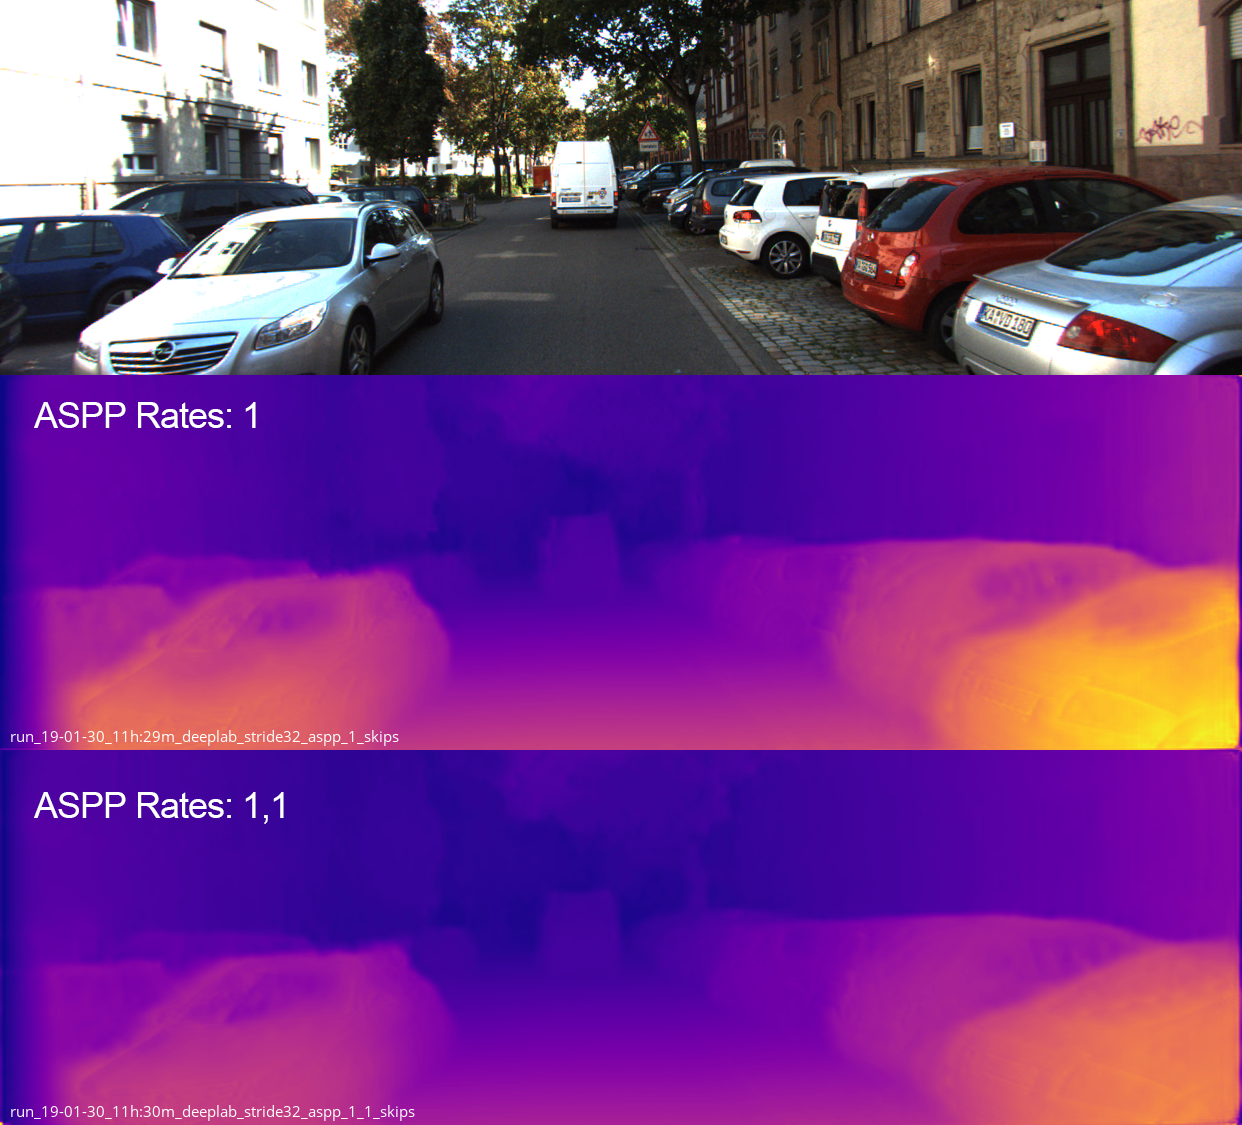
\includegraphics[width=0.7\textwidth]{figures/images/asppconvcomparison_001.png}
\end{frame}

\begin{frame}[c]{\subsecname: Atrous Rates (Visual Comparison)}
  \centering
  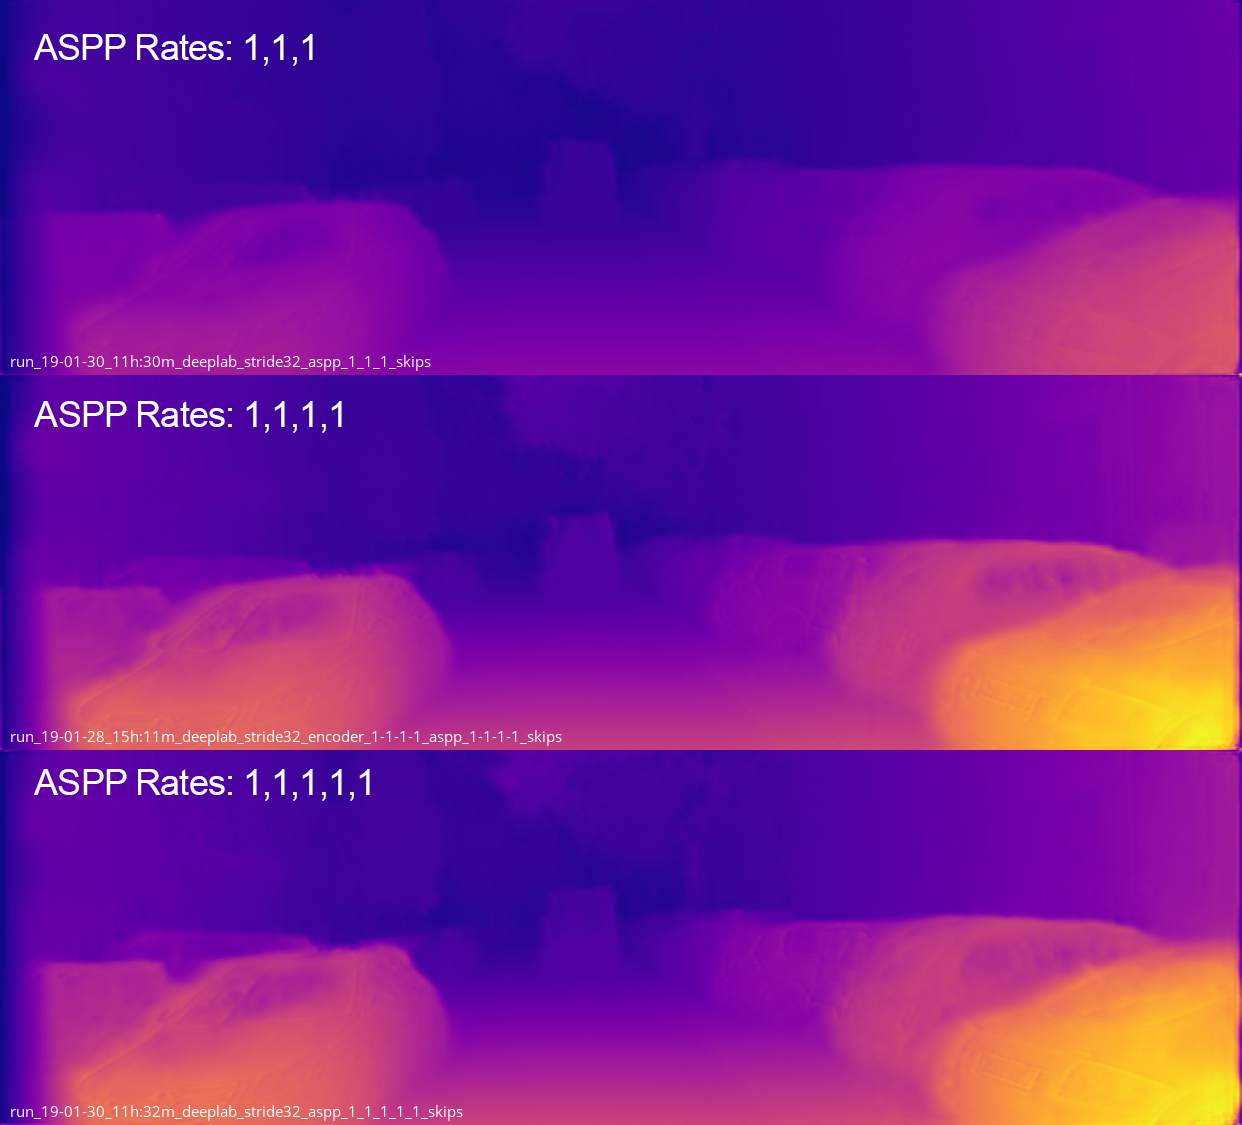
\includegraphics[width=0.7\textwidth]{figures/images/asppconvcomparison_002.png}
\end{frame}



\begin{frame}[c]{\subsecname: Atrous Rates (Squared relative error)}
  \centering
  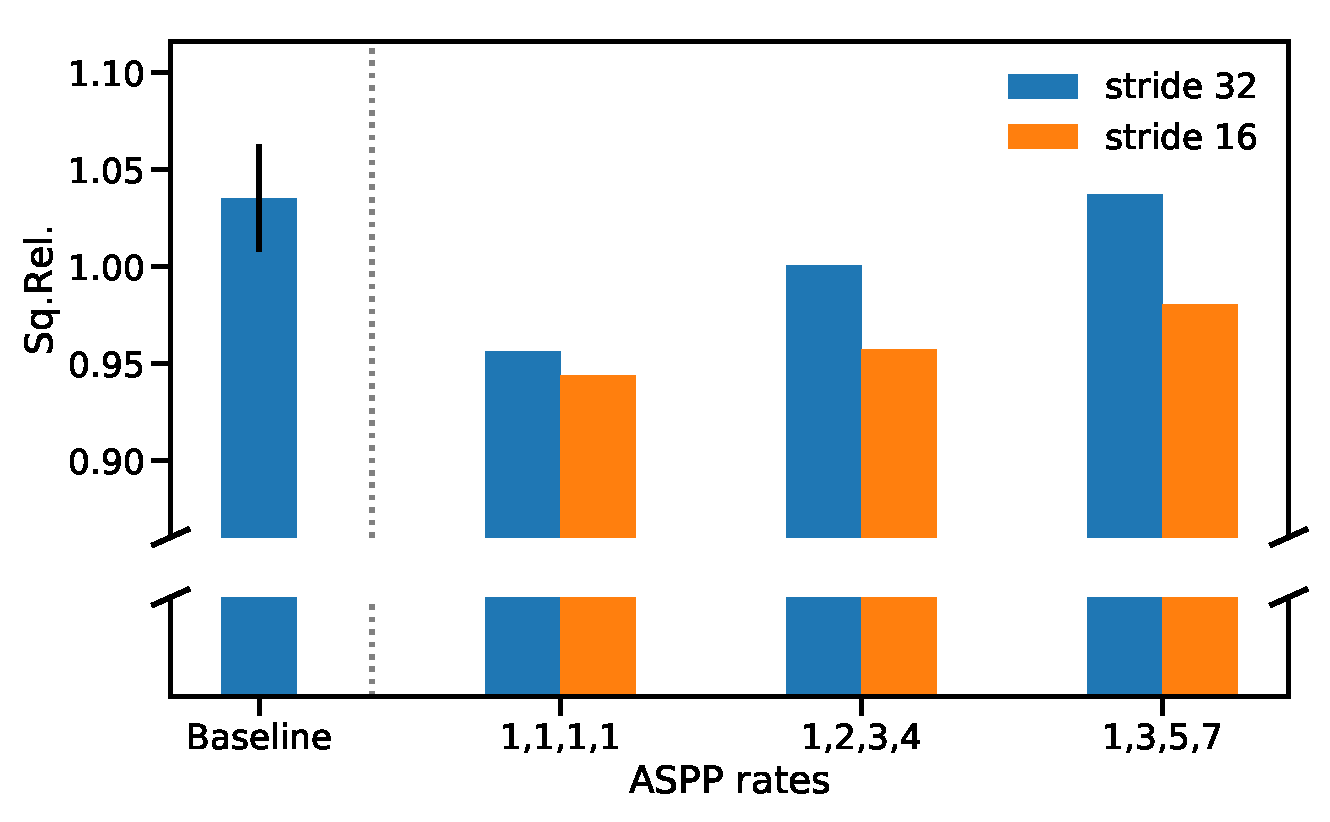
\includegraphics[width=1.0\textwidth]{figures/results/experiment1_SqRel.pdf}
\end{frame}

\begin{frame}[c]{\subsecname: Atrous Rates (RMSE)}
  \centering
  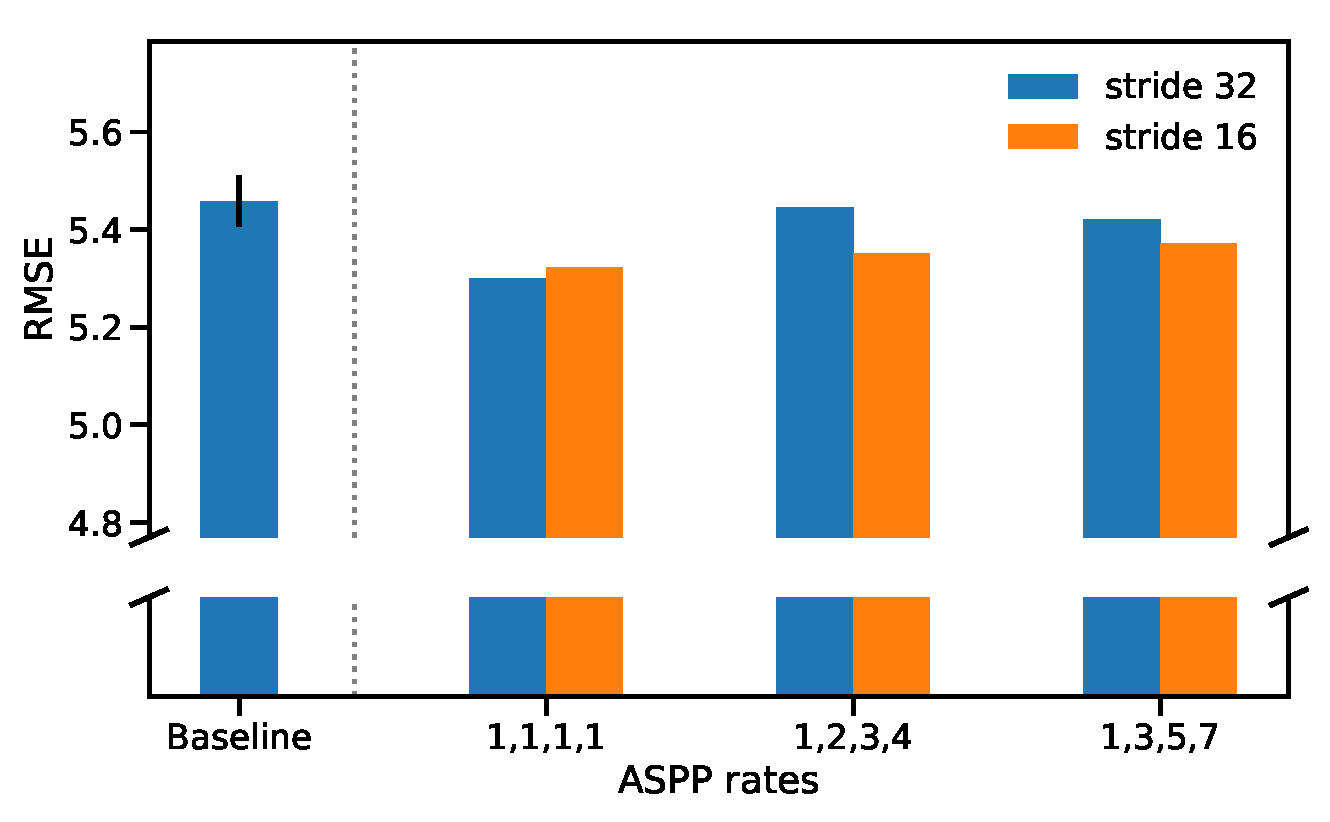
\includegraphics[width=1.0\textwidth]{figures/results/experiment1_RMSE.pdf}
\end{frame}

\begin{frame}[c]{\subsecname: Atrous Rates (RMSE of log)}
  \centering
  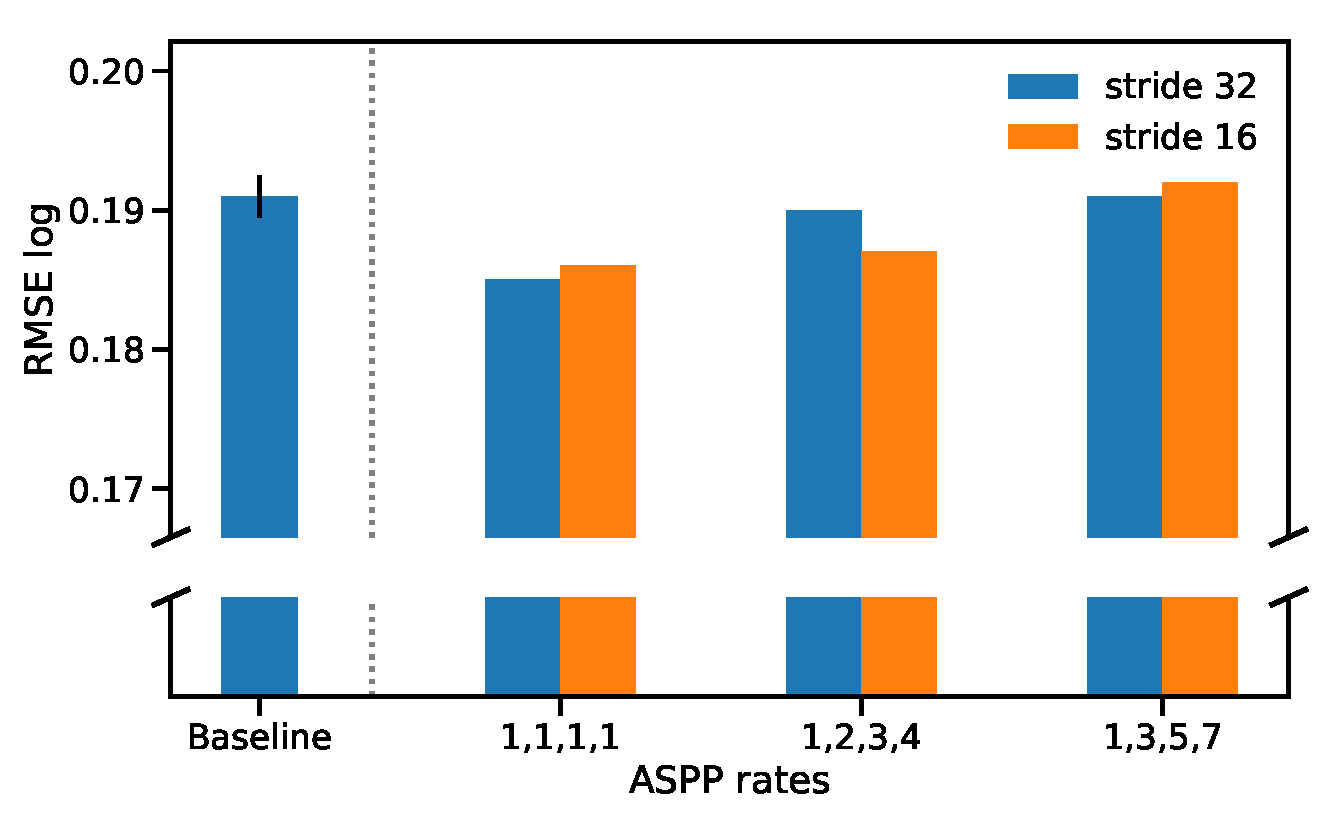
\includegraphics[width=1.0\textwidth]{{figures/results/experiment1_RMSE log}.pdf}
\end{frame}

\begin{frame}[c]{\subsecname: Atrous Rates (\% inliers 1)}
  \centering
  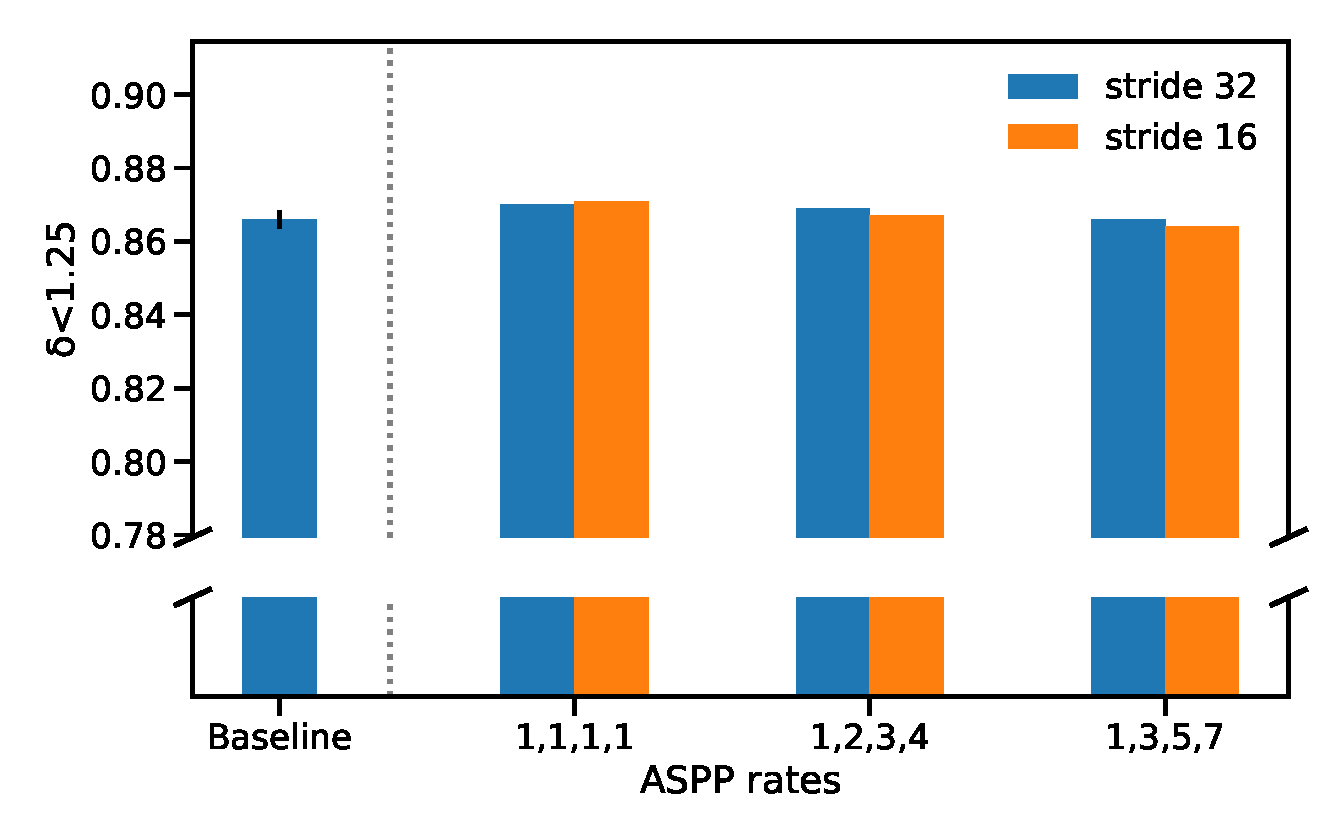
\includegraphics[width=1.0\textwidth]{{figures/results/experiment1_d<125}.pdf}
\end{frame}

\begin{frame}[c]{\subsecname: Atrous Rates (\% inliers 2)}
  \centering
  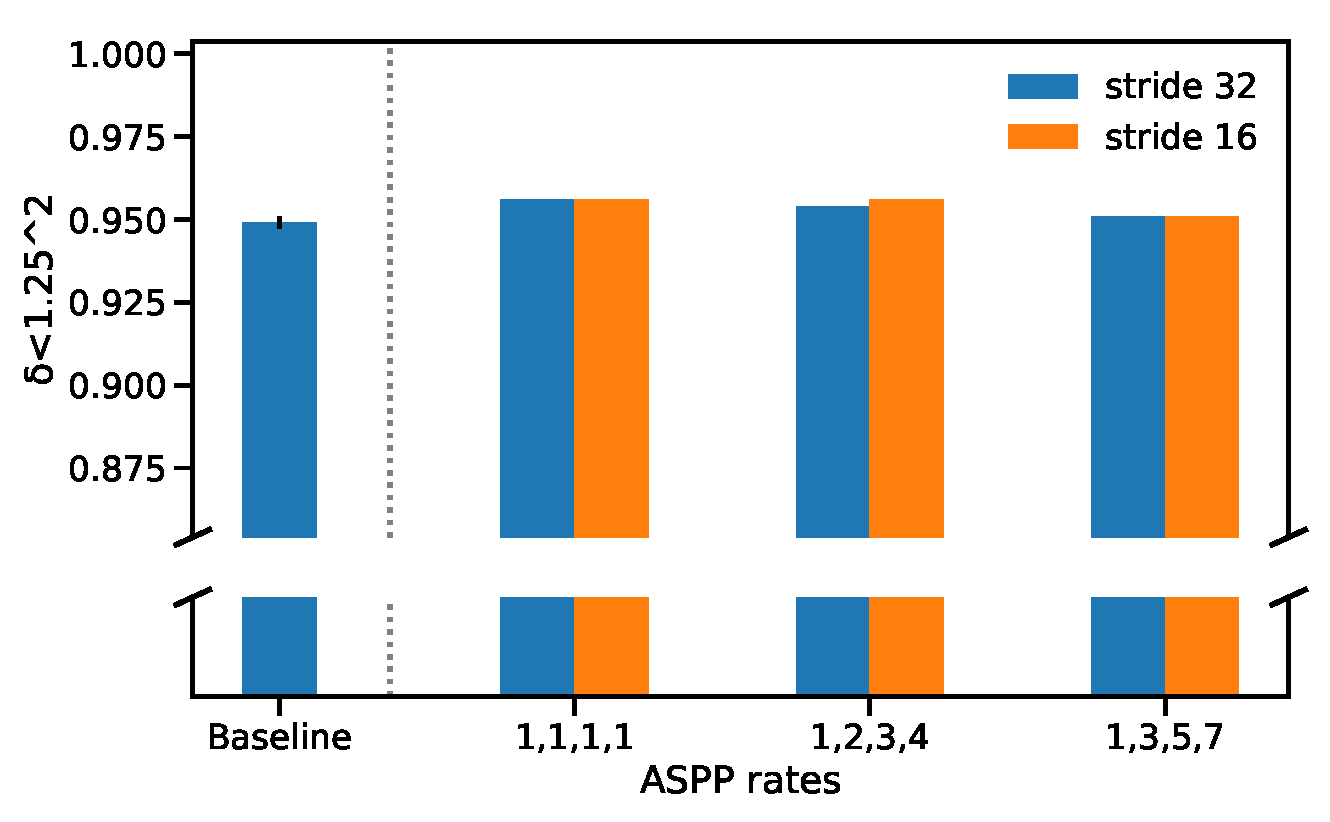
\includegraphics[width=1.0\textwidth]{figures/results/experiment1_d<125^2.pdf}
\end{frame}

\begin{frame}[c]{\subsecname: Atrous Rates (\% inliers 3)}
  \centering
  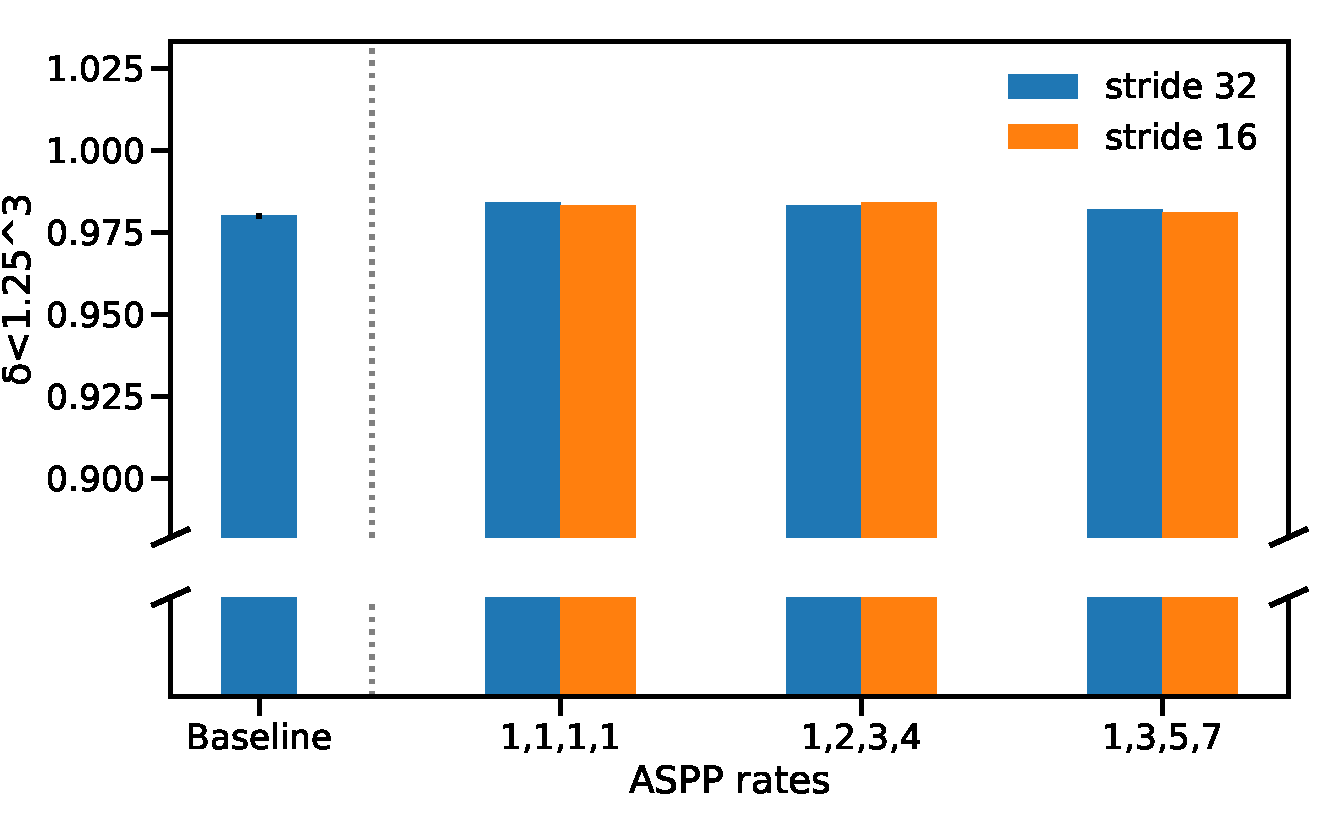
\includegraphics[width=1.0\textwidth]{figures/results/experiment1_d<125^3.pdf}
\end{frame}

\begin{frame}[c]{\subsecname: Atrous Rates (Squared relative error)}
  \centering
  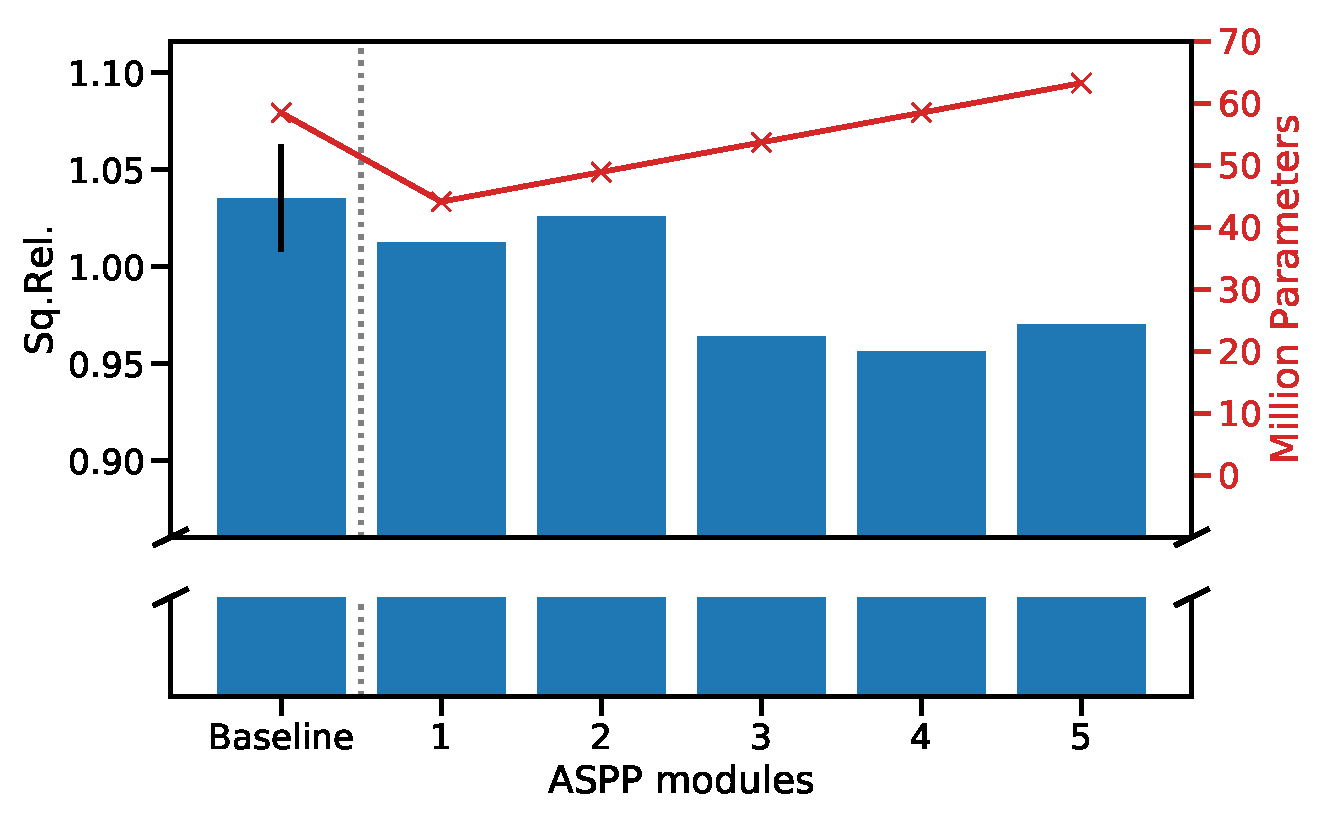
\includegraphics[width=1.0\textwidth]{figures/results/experiment2_SqRel.pdf}
\end{frame}

\begin{frame}[c]{\subsecname: Atrous Rates (RMSE)}
  \centering
  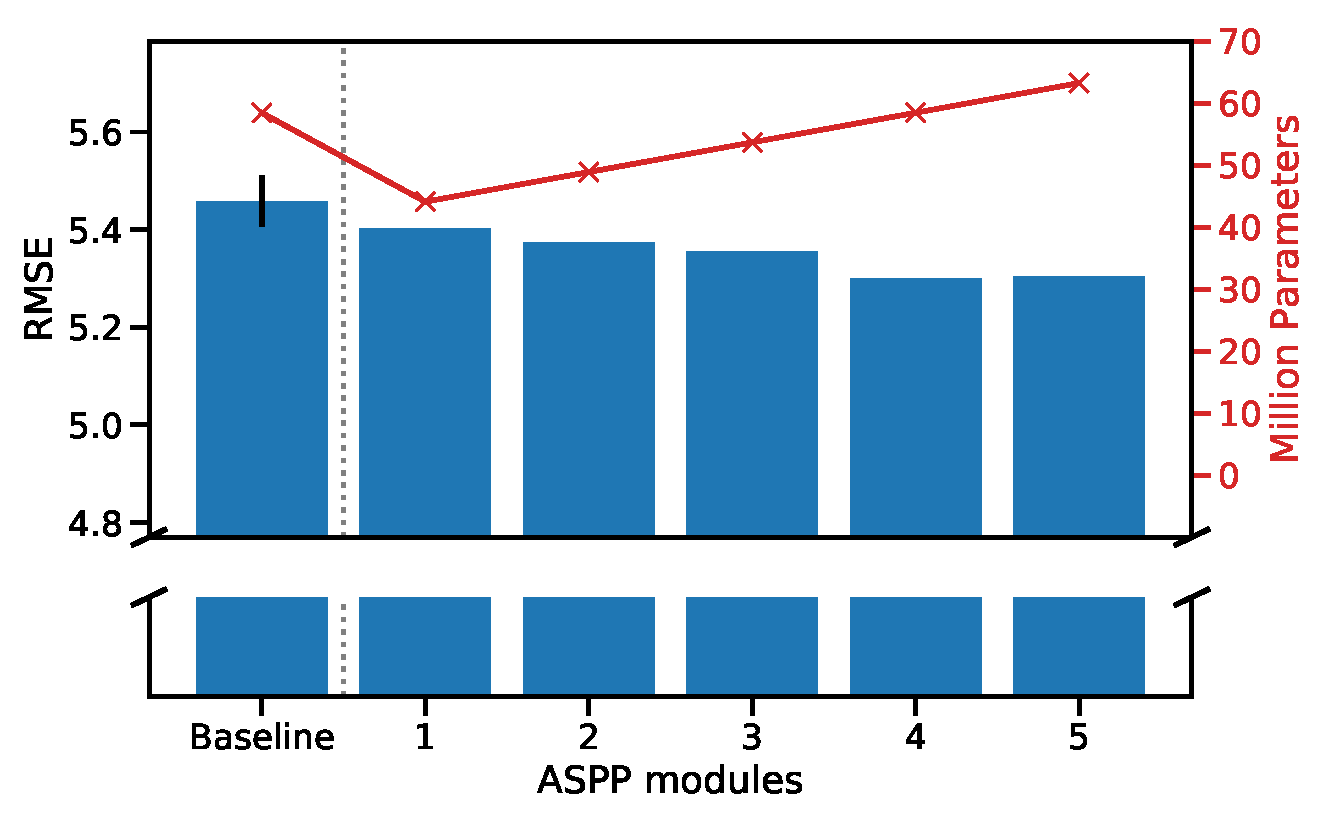
\includegraphics[width=1.0\textwidth]{figures/results/experiment2_RMSE.pdf}
\end{frame}

\begin{frame}[c]{\subsecname: Atrous Rates (RMSE of log)}
  \centering
  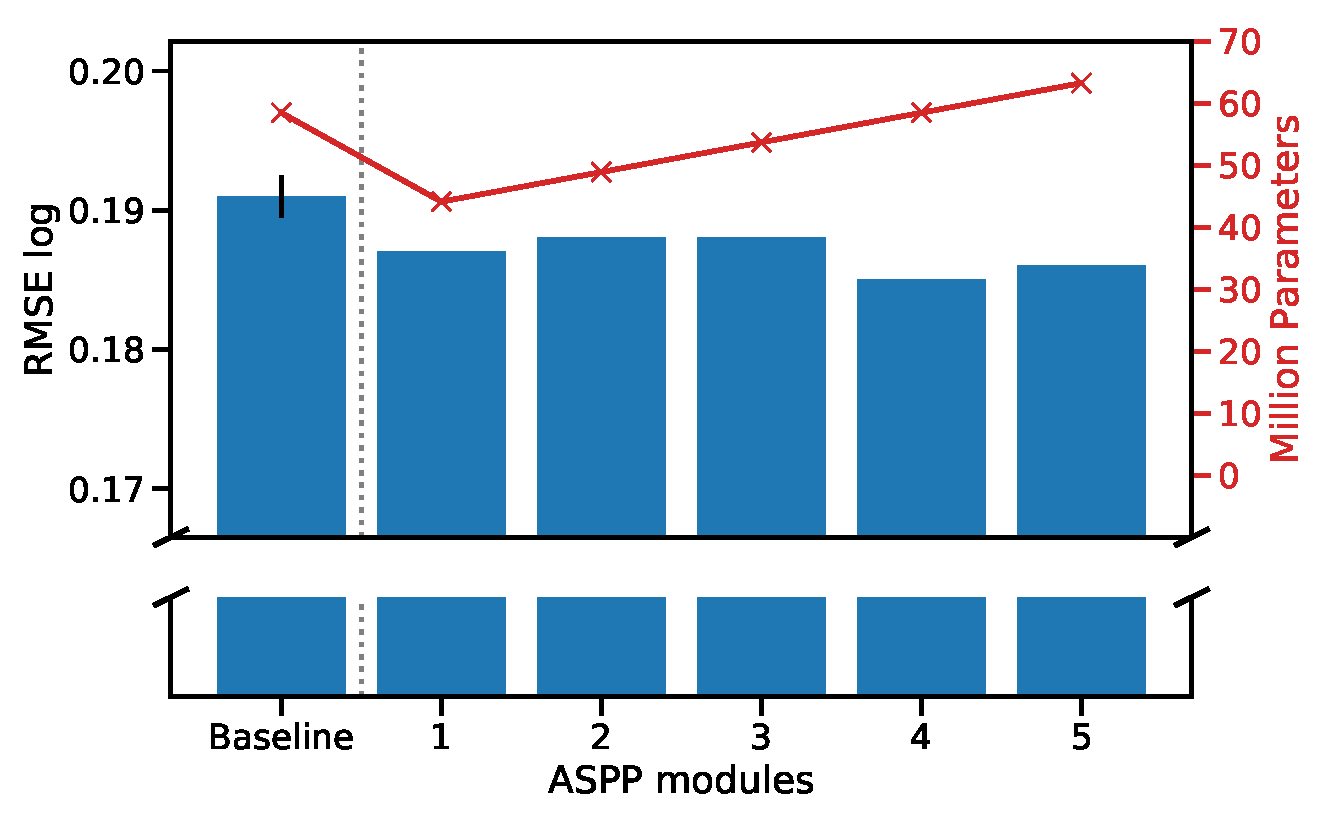
\includegraphics[width=1.0\textwidth]{figures/results/experiment2_RMSE log.pdf}
\end{frame}

\begin{frame}[c]{\subsecname: Atrous Rates (\% inliers 1)}
  \centering
  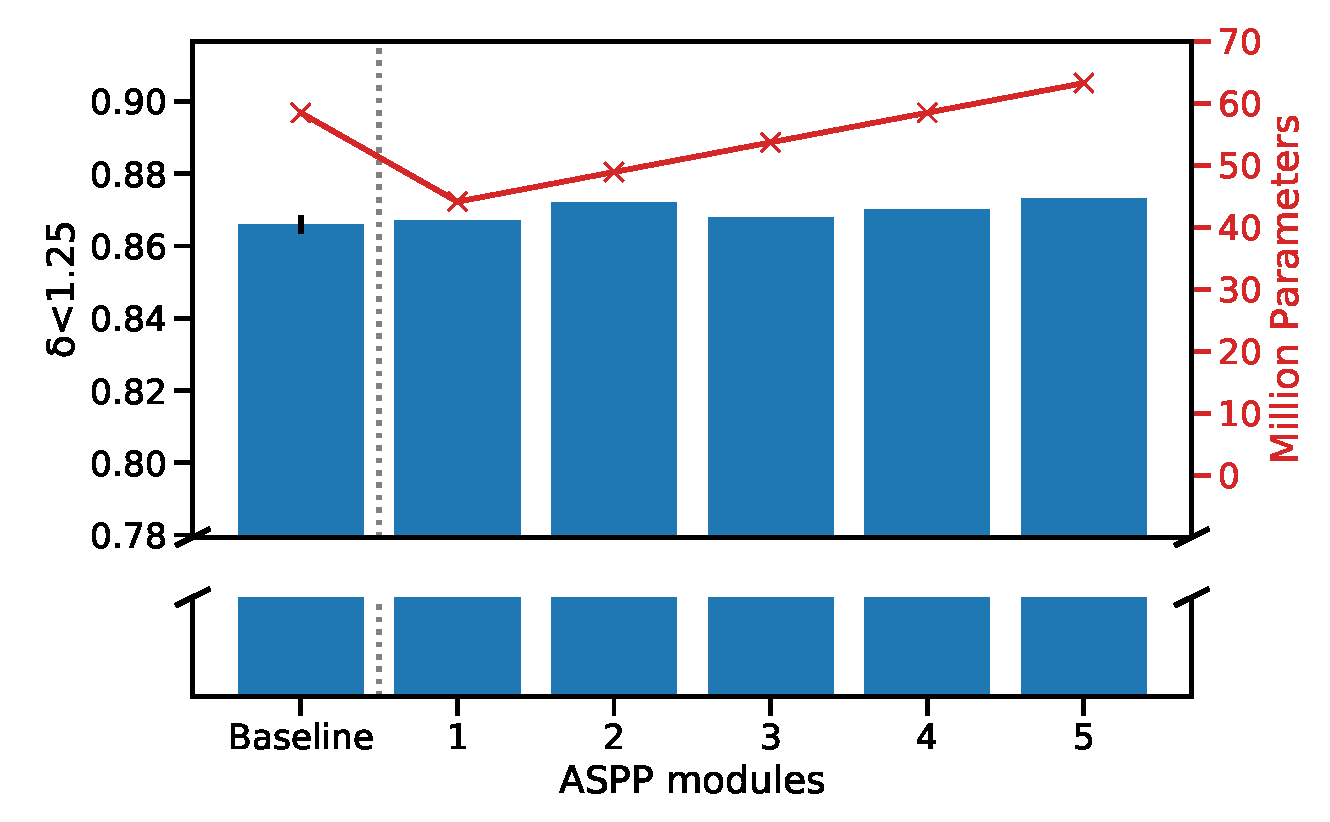
\includegraphics[width=1.0\textwidth]{figures/results/experiment2_d-125.pdf}
\end{frame}

\begin{frame}[c]{\subsecname: Atrous Rates (\% inliers 2)}
  \centering
  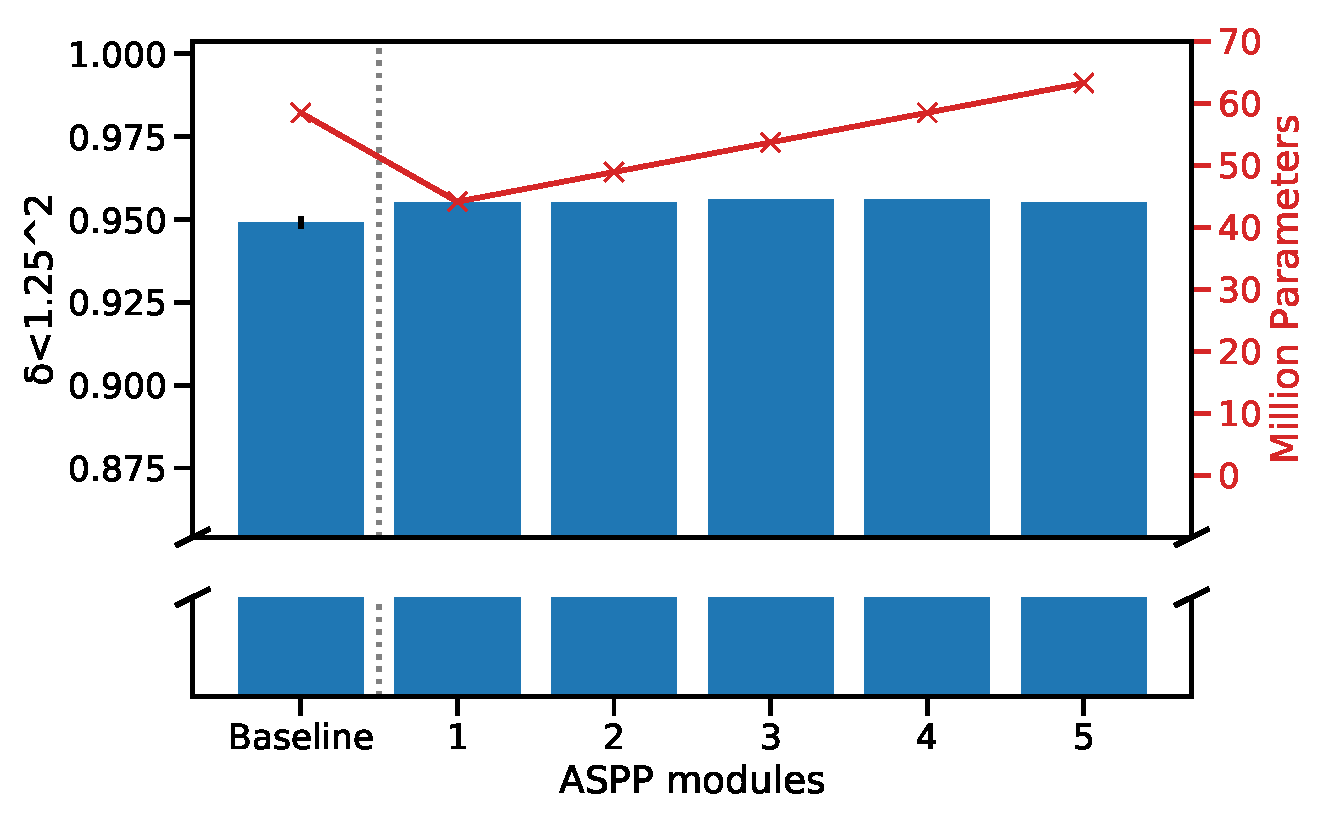
\includegraphics[width=1.0\textwidth]{figures/results/experiment2_d-125^2.pdf}
\end{frame}

\begin{frame}[c]{\subsecname: Atrous Rates (\% inliers 3)}
  \centering
  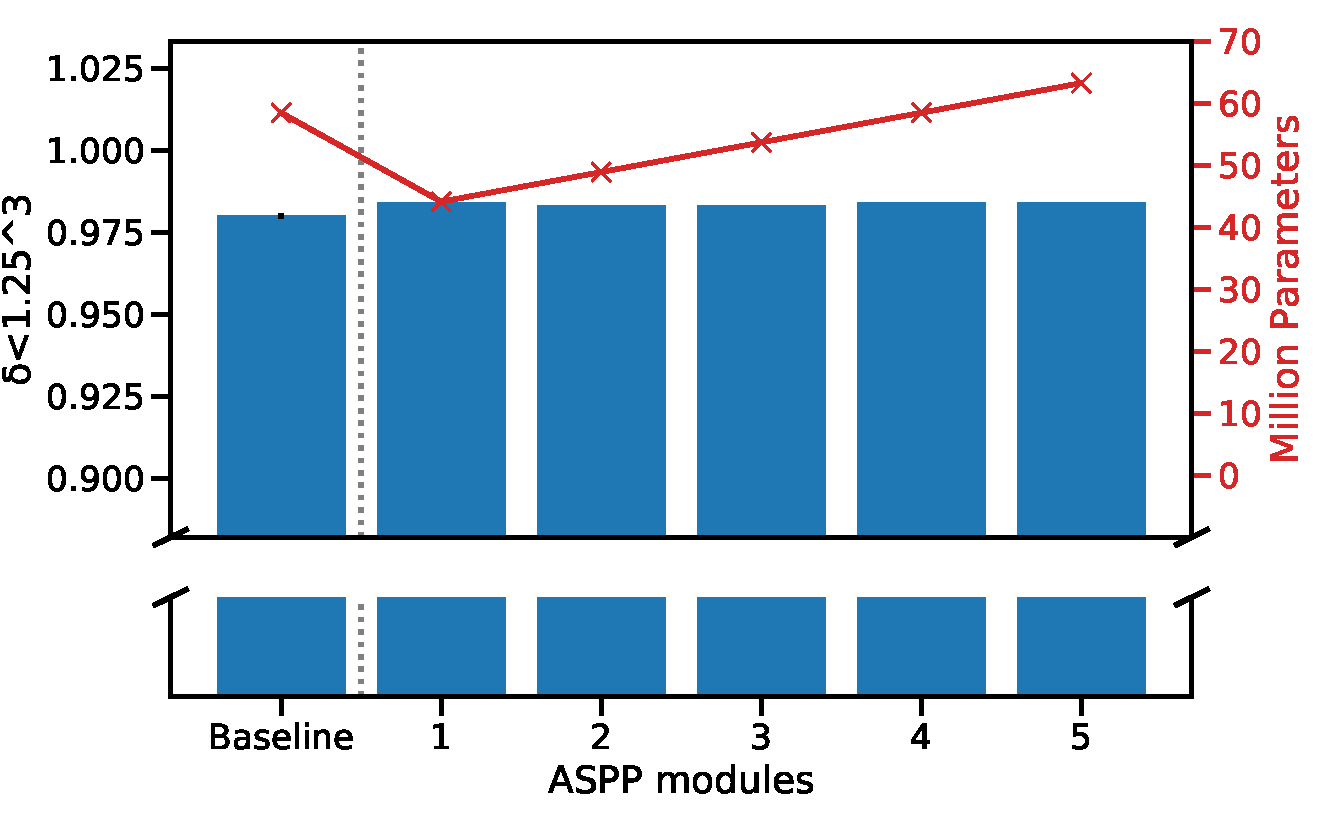
\includegraphics[width=1.0\textwidth]{figures/results/experiment2_d-125^3.pdf}
\end{frame}


\begin{frame}[c]{\subsecname: Output Stride Comparison}
  \centering
  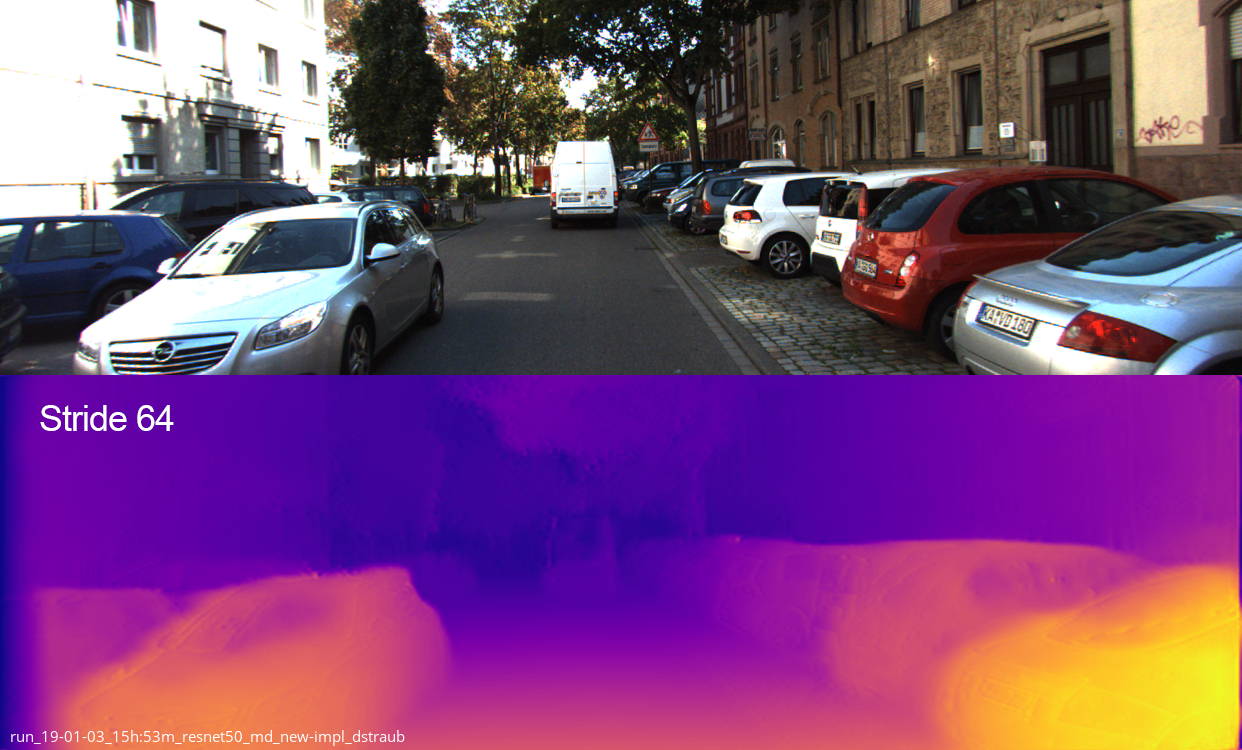
\includegraphics[width=1.0\textwidth]{figures/images/stridecomparison_001.png}
\end{frame}

\begin{frame}[c]{\subsecname: Output Stride Comparison}
  \centering
  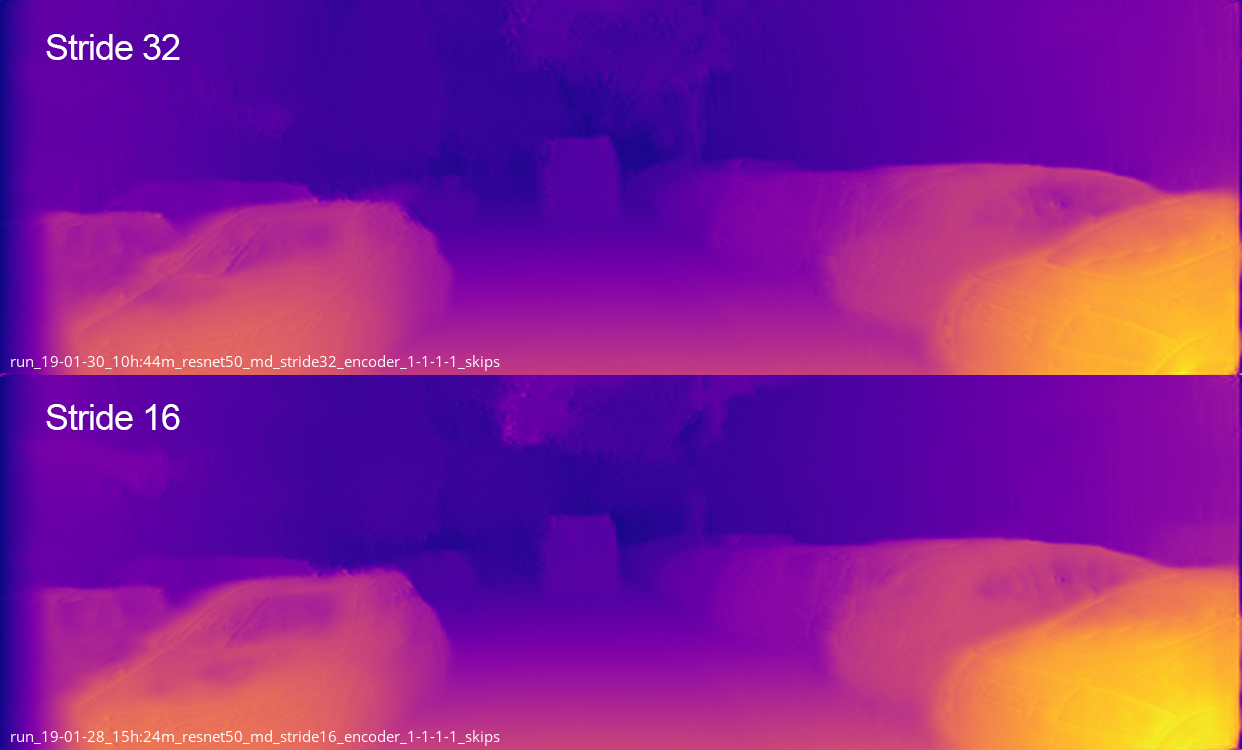
\includegraphics[width=1.0\textwidth]{figures/images/stridecomparison_002.png}
\end{frame}

\begin{frame}[c]{\subsecname: ASPP vs. no ASPP (without Skip Connections)}
\centering
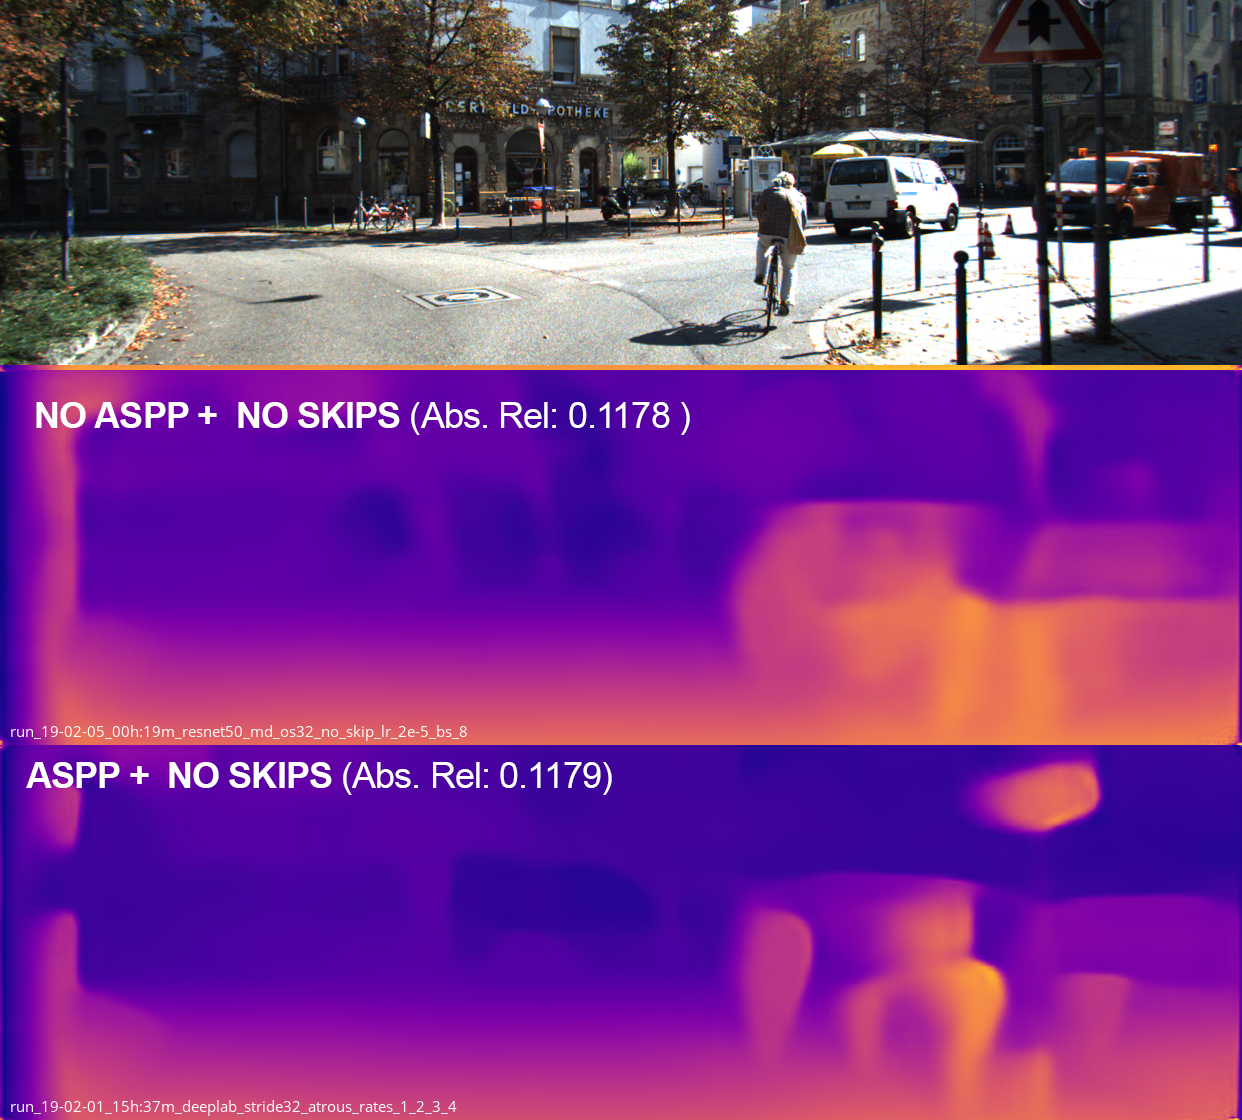
\includegraphics[width=0.7\textwidth]{figures/images/skipsvsnoskips2_error.png}
\end{frame}







% Uncomment if a bibliography is needed
% \bibliographystyle{plainnat}
% \bibliography{Master}
\end{document}
